\setcounter{chapter}{3}
\chapter[Learning from successes, not catastrophe: Using counterfactual analysis to highlight successful disaster risk reduction intervention]{Learning from successes, not catastrophe: Using counterfactual analysis to highlight successful disaster risk reduction intervention}\label{chap-counterfactual}

\begin{small}
\\
Chapter 4 is a journal article published as follows. Appendix \ref{app-pls-1} pertains to the Supplementary Material published with the paper.
\\ \\
\noindent
    \textbf{Rabonza M.L.}, Lin Y.C. and Lallemant D. (2022) Learning From Success, Not Catastrophe: Using Counterfactual Analysis to Highlight Successful Disaster Risk Reduction Interventions. \textit{Front. Earth Sci.} 10:847196. doi: 10.3389/feart.2022.847196
\\
\\
In addition, this chapter cites the following first-author paper, which is included in Appendix \ref{app-pls-2}. The paper presents the concept of four situations in which disaster risk reduction interventions go un-noticed. Two out of the four situations are addressed in Chapter 4's case studies.
\\
\\
\noindent
\textbf{Rabonza, M.L.}, Lallemant,  D.,  Lin,  Y. C., Tadepalli,  S., Wagenaar,  D., Nguyen,  M., Choong,  J., Liu,  C. J. N., Sarica,  G. M., Widawati,  B. A. M., Balbi,  M., Khan,  F., Loos,  S. \& Lim,  T. N. (2022). Shedding light on avoided disasters : measuring the invisible benefits of disaster risk management using probabilistic counterfactual analysis. \textit{A contributing paper to the United Nations Office for Disaster Risk Reduction (UNDRR) Global Assessment Report 2022}. https://www.undrr.org/publication/shedding-light-avoided-disasters-measuring-invisible-benefits-disaster-risk-reduction

% \label{app-pls-1}

%----------------
% \section*{Highlights}
% %--- RESEARCH HIGHLIGHTS
% %----------------
% \begin{itemize}

% \item I combine probabilistic risk analysis and counterfactual analysis to quantify and highlight the benefits of risk reduction that often go unnoticed.

% \item I estimate the benefits of an intervention in a past earthquake, and for a hazard that has not yet occurred.

% \item I highlight the success of the seismic retrofitting program for schools in Nepal during the 2015 Gorkha earthquake, and the benefits of scaling up the program.

% \end{itemize}


%%% Start of highlights
\clearpage
\vspace*{\fill}
\begingroup
\centering

\textbf{\Large{Chapter highlights}}

\hrulefill 

\begin{itemize}
\item \textsl{I combine probabilistic risk analysis and counterfactual analysis to quantify and highlight the benefits of risk reduction that often go unnoticed.}

\item \textsl{I estimate the benefits of an intervention in a past earthquake, and for a hazard that has not yet occurred.}

\item \textsl{I highlight the success of the seismic retrofitting program for schools in Nepal during the 2015 Gorkha earthquake, and the benefits of scaling up the program.}
\end{itemize}


\endgroup
\vspace*{\fill}


% %----------------
% \vspace{2cm}
% \noindent
% \textbf{Keywords:} Counterfactual analysis, Probabilistic risk, Disaster risk reduction, Risk framework, School earthquake safety

\end{small}
\clearpage



%%%%%%%%%%%%%%%%%
\section{Abstract}

In the aftermath of a disaster, news and research attention is focused almost entirely on catastrophic narratives and the various drivers that may have led to the disaster. Learning from failure is essential to preventing future disasters. However, hyperfixation on the catastrophe obscures potential successes at the local scale, which could serve as important examples and learning resources in effective risk mitigation. To highlight effective risk mitigation actions that would otherwise remain unnoticed, we propose the use of probabilistic downward counterfactual analysis. This approach uses counterfactual modelling of a past hazard event with consequences made worse (i.e. downward counterfactual) by the absence of the mitigation intervention. The approach follows probabilistic risk analysis procedures where uncertainties in the simulated events and outcomes are accounted for and propagated. We demonstrate the method using a case study of Nepal’s School Earthquake Safety Program, implemented before the 2015 $M_{w}$ 7.8 Gorkha earthquake. Using a school building database for Kathmandu Valley, Nepal, we present two applications: (1) the quantification of lives saved during the Gorkha earthquake as a result of the retrofitting of schools in Kathmandu Valley since 1999, (2) the quantification of the annual expected lives saved if the pilot retrofitting program was extended to all school buildings in Kathmandu Valley based on a probabilistic seismic hazard model. The shift in focus from realised outcome to counterfactual alternative enables the quantification of the benefits of risk reduction programs amidst disaster, or for a hazard that has yet to unfold. Such quantified counterfactual analysis can be used to celebrate successful risk reduction interventions, providing important positive reinforcement to decision-makers with political bravery to commit to the implementation of effective measures.


%%%%%%%%%%%%%%%%%%%%%%%%%%%%|
%%% INTRODUCTION
%%%%%%%%%%%%%%%%%%%%%%%%%%%%|
\section{Introduction}
\label{section-intro}

Success in disaster risk management (DRM) means that natural hazard events do not turn into disasters, and communities continue to function and be resilient to shocks and stresses from hazards. Since the extent of a disaster can be characterised by loss of life and disruptions to the physical, built and social environments, \citep{mileti1999disasters, smith2005through, moore1958tornadoes}, the extent of success of risk reduction interventions manifest primarily as reduced impact. As such, success is measured as an \textit{absence} (e.g. no damage, fewer casualties, etc). This poses a challenge for recognising and incentivising important investments in DRM interventions since they are made invisible by their very nature.

In the aftermath of earthquakes, storms, and floods, narratives of catastrophe dominate the interest of media, political and research communities. However, this hyper-fixation on the catastrophe can obscure important successes amid the broader disaster. Another challenge is to recognize successful interventions if the hazard they were designed for has not yet occurred. This happens when we rely on a disaster occurrence to make mitigation benefits visible. For extreme and rare hazard events, for example, the benefits of risk reduction may manifest only in the distant future. Because of the significant time delay between the interventions and their benefits being manifested, such interventions can be perceived as unsuccessful or squandered until the event occurs. These are two of the challenges described in \cite{lallemant_rabonza_gar_2022} where successful DRM interventions are made invisible: \textit{invisible success in the midst of broader disaster}, and \textit{invisible success due to yet unrealised benefits} (Full paper included as Supplementary in the Appendix). These \textit{invisible successes} of mitigation interventions are related to a cognitive tendency called \textit{outcome bias} - the tendency to judge the quality of a decision by the outcome alone \citep{robson_2019}. 

To address outcome bias, we propose a \textit{probabilistic downward counterfactual analysis} approach. It relies on comparing the outcome of a realised event in which a risk reduction was implemented, to an alternative branch of history (i.e. \textit{counterfactual}) in which the disaster risk reduction intervention was not implemented.  Throughout the paper, we use the term \textit{realised}  to refer to events or outcomes that transpired (in juxtaposition to counterfactual), in alignment with prior literature on probability and counterfactual analysis \citep{roese1997counterfactual}.  An imagined scenario where an intervention is absent is considered a \textit{downward counterfactual} because the assumed outcome is worse than what was observed in reality \citep{roese1997counterfactual}.  This is in contrast with an \textit{upward counterfactual} where the assumed outcome is better. Probabilistic downward counterfactual analysis is \textit{probabilistic} in that it follows probabilistic risk analysis procedures to propagate and account for uncertainties in events and outcomes. In this paper, we present two applications of probabilistic downward counterfactual analysis to highlight the effectiveness of risk reduction in terms of probabilistic lives saved. The first application estimates the benefits of an intervention in a past earthquake through comparison of fatalities modelled without the risk intervention and actual fatalities. The second application estimates the probabilistic benefits of a mitigation for a hazard that has not yet occurred. Instead of an actual past event, a hazard model is used to calculate the intervention's benefits.

The paper’s main contribution is in combining the probabilistic risk analysis framework and counterfactual analysis to calculate and highlight lives saved from successful disaster risk reduction interventions, that otherwise go unnoticed. The significance and novelty of this work is in shifting our perception of the benefits of risk reduction intervention, by using an appropriate counterfactual scenario as the baseline against which to calculate and judge these benefits. Rather than focusing entirely on realised outcomes, the analysis of counterfactual outcomes shines light on the value of a mitigation intervention by demonstrating what would have been without such intervention. Downward counterfactual risk analysis has only so far been used to identify potential worse impacts for the purpose of insurance, preparedness, or future mitigation \citep[e.g.][]{lin2020modeling, aspinall2019counterfactual, woo2019downward, woo2018counterfactual, shepherd2018storylines, woo2017reimagining, oughton2019stochastic, aspinall2019counterfactual}. This study pioneers a systematic approach to creating incentives for good decision-making on the basis of probabilistic risk. The quantification of probabilistic lives saved by effective risk reduction programs in a major hazard event serves as a powerful indicator of the intervention's success that would otherwise remain unnoticed amidst a disaster. In addition, the calculated probabilistic benefits of an intervention provide important incentive and encouragement to decision-makers committed to implementing effective measures even if the benefits are not materialized yet by the occurrence of a hazard event. Altogether, this work is a new domain of application of counterfactual analysis with much potential across the broad spectrum of hazards. 

The proposed framework has significant implications to multiple potential stakeholders. For policymakers, there is currently little political capital gained from investing in resilience if the benefits of such investments are invisible. By having the benefits of these investments visible to their constituents, policymakers will be incentivised for risk-informed decision-making. For donors and funders, this framework would enable them to monitor progress in terms of probabilistic impacts reduced, even if such benefits remain unrealized until a disaster strikes. For disaster risk management practitioners, while it is important to learn from failures, it is equally important to learn from successes, and share them broadly so they can be emulated, scaled, and adapted in other contexts where they are needed. Importantly, it also provides a mechanism to recognise and elevate the important, humble, long-term, and dedicated work conducted by many to keep our communities safe, even when their work is unseen.

The paper is organized as follows. Section \ref{section-counter} introduces the proposed framework in the context of probabilistic risk analysis. In Section \ref{section-retrofit-program}, we describe the earthquake risk intervention that will be the focus of our two applications: the school earthquake retrofitting program in Nepal, implemented before the 2015 $M_{w}$ 7.8 Gorkha earthquake. In the subsequent sections, we present the methods (Section \ref{section-methods}) and two applications (Section \ref{section-apps}) that shed light on the benefits of the retrofitting program. The first application estimates the number of lives saved during the Gorkha earthquake as a result of the retrofitting of schools in Kathmandu Valley since 1997. The second application calculates the annual expected lives saved if the retrofitting program was extended to all school buildings based on a probabilistic seismic hazard model we generated for Kathmandu Valley, Nepal. This is followed by Discussion (Section \ref{section-discussion}) and Conclusion (Section \ref{section-conclusion}).


%%%%%%%%%%%%%%%%%%%%%%%%%%%%|%%%%%%%%%%%%%%%%%%%%%%%%%%%%|
%%% COUNTERFACTUAL ANALYSIS
%%%%%%%%%%%%%%%%%%%%%%%%%%%%|%%%%%%%%%%%%%%%%%%%%%%%%%%%%|
\section{Counterfactual risk analysis framework}
\label{section-counter}

The main idea of counterfactual disaster risk analysis is to explore alternative branches of history to assess past situations where a disaster might have occurred but was averted or failed to materialise \citep{woo2018counterfactualvar}. Impacts associated with a past event, i.e. a realised event, can be expressed as the function of the (a) Hazard, the likelihood of potentially damaging events, (b) Exposure, the characteristics of assets such as people, buildings and infrastructure and (c) Vulnerability, the susceptibility of the exposed assets to sustain impact for a given hazard intensity \citep{UNISDRterms2009}. Then, we can write the losses from the realised event as 

\begin{equation}\label{eq:realised}
        I_{realised} = f \left( \theta_H, \theta_E, \theta_V \right),
    \end{equation}
where $\theta_H$, $\theta_E$, and $\theta_V$ are the hazard, exposure and vulnerability parameters consecutively. Modifications ($\delta_.$) of one or multiple parameters that define the realised event allow one to define the impact of a counterfactual event:

\begin{equation}\label{eq:counterfactual_risk}
    I_{counterfactual} = f \left( \theta_H + \delta_H,  \theta_E + \delta_E,  \theta_V + \delta_V \right),
    \end{equation}

The purpose of the deviations, $\delta_H$, $\delta_E$, and $\delta_V$, to the realised event’s parameters is to explore counterfactuals. $\delta_H$ helps us explore counterfactuals in the hazard (e.g. what if the earthquake had occurred at a slightly different location, or with opposite directivity of rupture?). $\delta_E$ helps us explore counterfactuals in the exposure (e.g. what if the 1906 San Francisco earthquake were to hit today’s building stock?). $\delta_V$ helps us explore counterfactuals in vulnerability (e.g. what if all unreinforced masonry buildings had been retrofitted?). In this paper, we focus on $\delta_V$, while $\delta_H$ and $\delta_E=0$, to highlight the value of effective vulnerability reduction programs that often go unnoticed.

Modelling the impact of events with either Equation \ref{eq:realised} or \ref{eq:counterfactual_risk} relies on probabilistic risk analysis. Traditionally used in engineering reliability assessments and performance-based design, probabilistic risk analysis has been an established approach to assess the risks from natural hazards to entire regions and cities \citep{pate2002risk, stergiou2010risk}. Probabilistic risk analysis systemically quantifies the potential impacts of hazard events on a system and the likelihood that such consequences would occur \citep{bedford2001probabilistic}. In the case of Equations 1 and 2, the impacts $I_{realised}$ and $I_{counterfactual}$ and their likelihood are obtained through the joint probability of the risk parameters.

The expected benefits ($B$) of effective risk mitigation is then calculated as the difference between the expected value (the mean) of impacts of the realised event $E(I_{realised})$ and the counterfactual event $E(I_{counterfactual})$ (see Equation \ref{eq:benefits} and Figure \ref{fig:conceptual_diagram}). Assuming the realised impacts are less than those of the counterfactual, $B$ is expected to be a positive value in Equation \ref{eq:benefits}.
    \begin{equation} \label{eq:benefits}
        B = E(I_{counterfactual}) - E(I_{realised})
    \end{equation}


\begin{figure}[h!] 
\begin{center}
    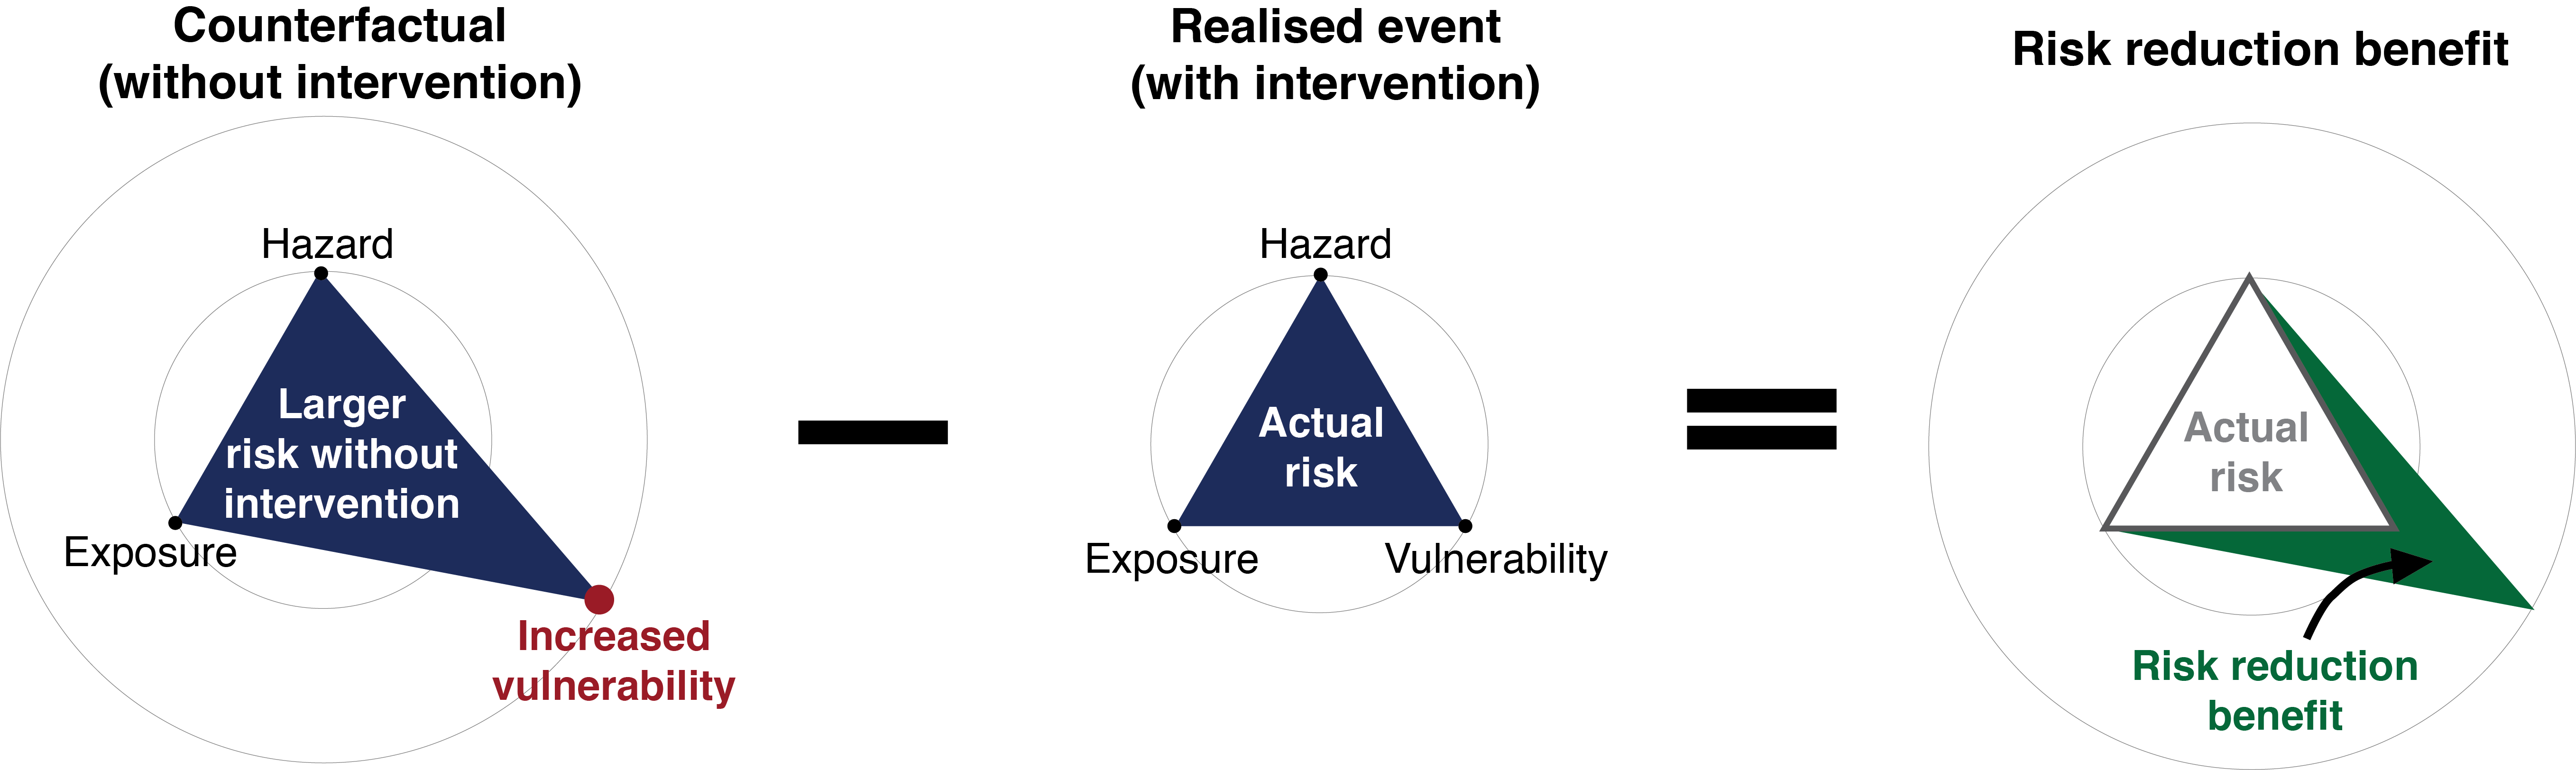
\includegraphics[width=\textwidth]{Figures/concept-diagram_rev2.png}
    \caption{The concept of the counterfactual risk analysis framework for quantifying the probabilistic benefits of effective risk reduction. This graphic serves as a demonstration of the framework that is specific for a risk intervention that reduces vulnerability.}
    \label{fig:conceptual_diagram}
\end{center}
\end{figure}

%%%%%%%%%%%%%%%%%%%%%%%%%%%%|%%%%%%%%%%%%%%%%%%%%%%%%%%%%|
%%% SCHOOLS RETROFIT
%%%%%%%%%%%%%%%%%%%%%%%%%%%%|%%%%%%%%%%%%%%%%%%%%%%%%%%%%|
\section{Invisible success of seismically retrofitting schools in Nepal}
\label{section-retrofit-program}

In this paper, we implement the proposed framework to highlight invisible benefits of effective earthquake risk mitigation. Specifically, we focus on one of the most significant risk interventions in recent years that led to improved construction practices - the seismic retrofitting of school buildings in Nepal. Amid the destruction and tragic loss during the Gorkha earthquake, the life-saving benefit of the school retrofitting was obscured. Likewise if an earthquake event has not yet occurred, retrofitting program may seem like a waste even though an earthquake may occur at any time. Probabilistic counterfactual risk analysis can be used to shed light on these invisible benefits.

School buildings in Nepal are recognized to be at high risk amidst the region's high seismicity from the convergence of the Indian tectonic plate with the Eurasian plate, and due to informal construction practices done with little engineering guidance \citep{marasini2020}. Damage to school buildings was extensive from large earthquakes in recent history - the 1988 $M_{w}$ 6.6 Udayapur earthquake \citep{gupta1988report}, and the 2011 $M_{w}$ 6.9 Sikkim/Nepal border earthquake \citep{rai2012reconnaissance}. The 2015 Gorkha earthquake is a unique example in terms of the impacts on schools because the earthquake happened on a Saturday, whilst the school was not in session. Had the earthquake hit on a school day, over one million students would have been affected \citep{dixit2014public}.

Seismic retrofitting of school buildings started in 1997 through the leadership of the National Society for Earthquake Technology (NSET) as part of Nepal's School Earthquake Safety Program (SESP)  \citep{marasini_2019}. By the time of the Gorkha earthquake in 2015, 300 schools had been retrofitted, 160 of which were in Kathmandu Valley. It was a big achievement that none of the schools retrofitted under SESP collapsed or needed major repairs after the earthquake. Because the buildings were found to be structurally sound, all the retrofitted buildings served as safe shelters and required fewer temporary classrooms \citep{marasini_2019}. 
Following the direction of SESP towards safe learning facilities, the Government of Nepal aims to achieve minimum school safety criteria nationwide by 2030 through the Comprehensive School Safety Master Plan developed by Nepal's Ministry of Education, Science and Technology \citep{cehrdc2018} based on the global Comprehensive School Safety Framework \citep{unisdr2017}. Recognizing the need to strengthen more than 60,000 school buildings all over Nepal \citep{marasini2020}, one of the activities in the Master Plan is to retrofit school buildings in earthquake-affected areas.

%%%%%%%%%%%%%%%%%%%%%%%%%%%%|%%%%%%%%%%%%%%%%%%%%%%%%%%%%|
%%% METHODS
%%%%%%%%%%%%%%%%%%%%%%%%%%%%|%%%%%%%%%%%%%%%%%%%%%%%%%%%%|
\section{Methods}
\label{section-methods}

\subsection{School building database}
% reference to a map?
The analyses in this paper are carried out on a database of Nepalese school buildings surveyed and georeferenced in 2013 through the partnership of the Open Data for Resilience Initiative (OpenDRI) and the Government of Nepal with support from Kathmandu Living Labs \citep{opendri_2012}. The building database covers Kathmandu Valley and was produced to understand the seismic risk in the education and health infrastructure. Parts in the dataset related to educational infrastructure were tagged as either \textit{school}, \textit{college}, \textit{university}, or \textit{kindergarten}. The database provides information on the location, number of daytime occupants on a school day, structure type, and whether the school building was retrofitted or not. We chose the OpenDRI dataset for this paper because these building attributes allow us to determine which school buildings were retrofitted under SESP before the 2015 Gorkha earthquake. In addition, the buildings’ structure type can be used to identify the buildings’ vulnerability, while the number of daytime occupants can be used for fatality calculations.

After screening the raw OpenDRI dataset for missing information or non-school buildings, the final dataset we use for this work consists of 5029 school buildings, of which 70 were retrofitted (see Figure \ref{fig:data-all}). We highlight that the OpenDRI dataset we use for this study provides information on only 70 out of the 160 retrofitted school buildings identified by NSET in Kathmandu Valley's affected areas \citep{marasini_2019}. The database consists of buildings with unreinforced masonry-type (URM-type) and reinforced concrete-type (RC-type) structures. The daytime occupancy for the 70 retrofitted schools go up to 800, with a mean of 134, whereas the occupancy for the 5029 school buildings go up to 2000 with a mean of 120.

\begin{figure}[h!] 
\begin{center}
    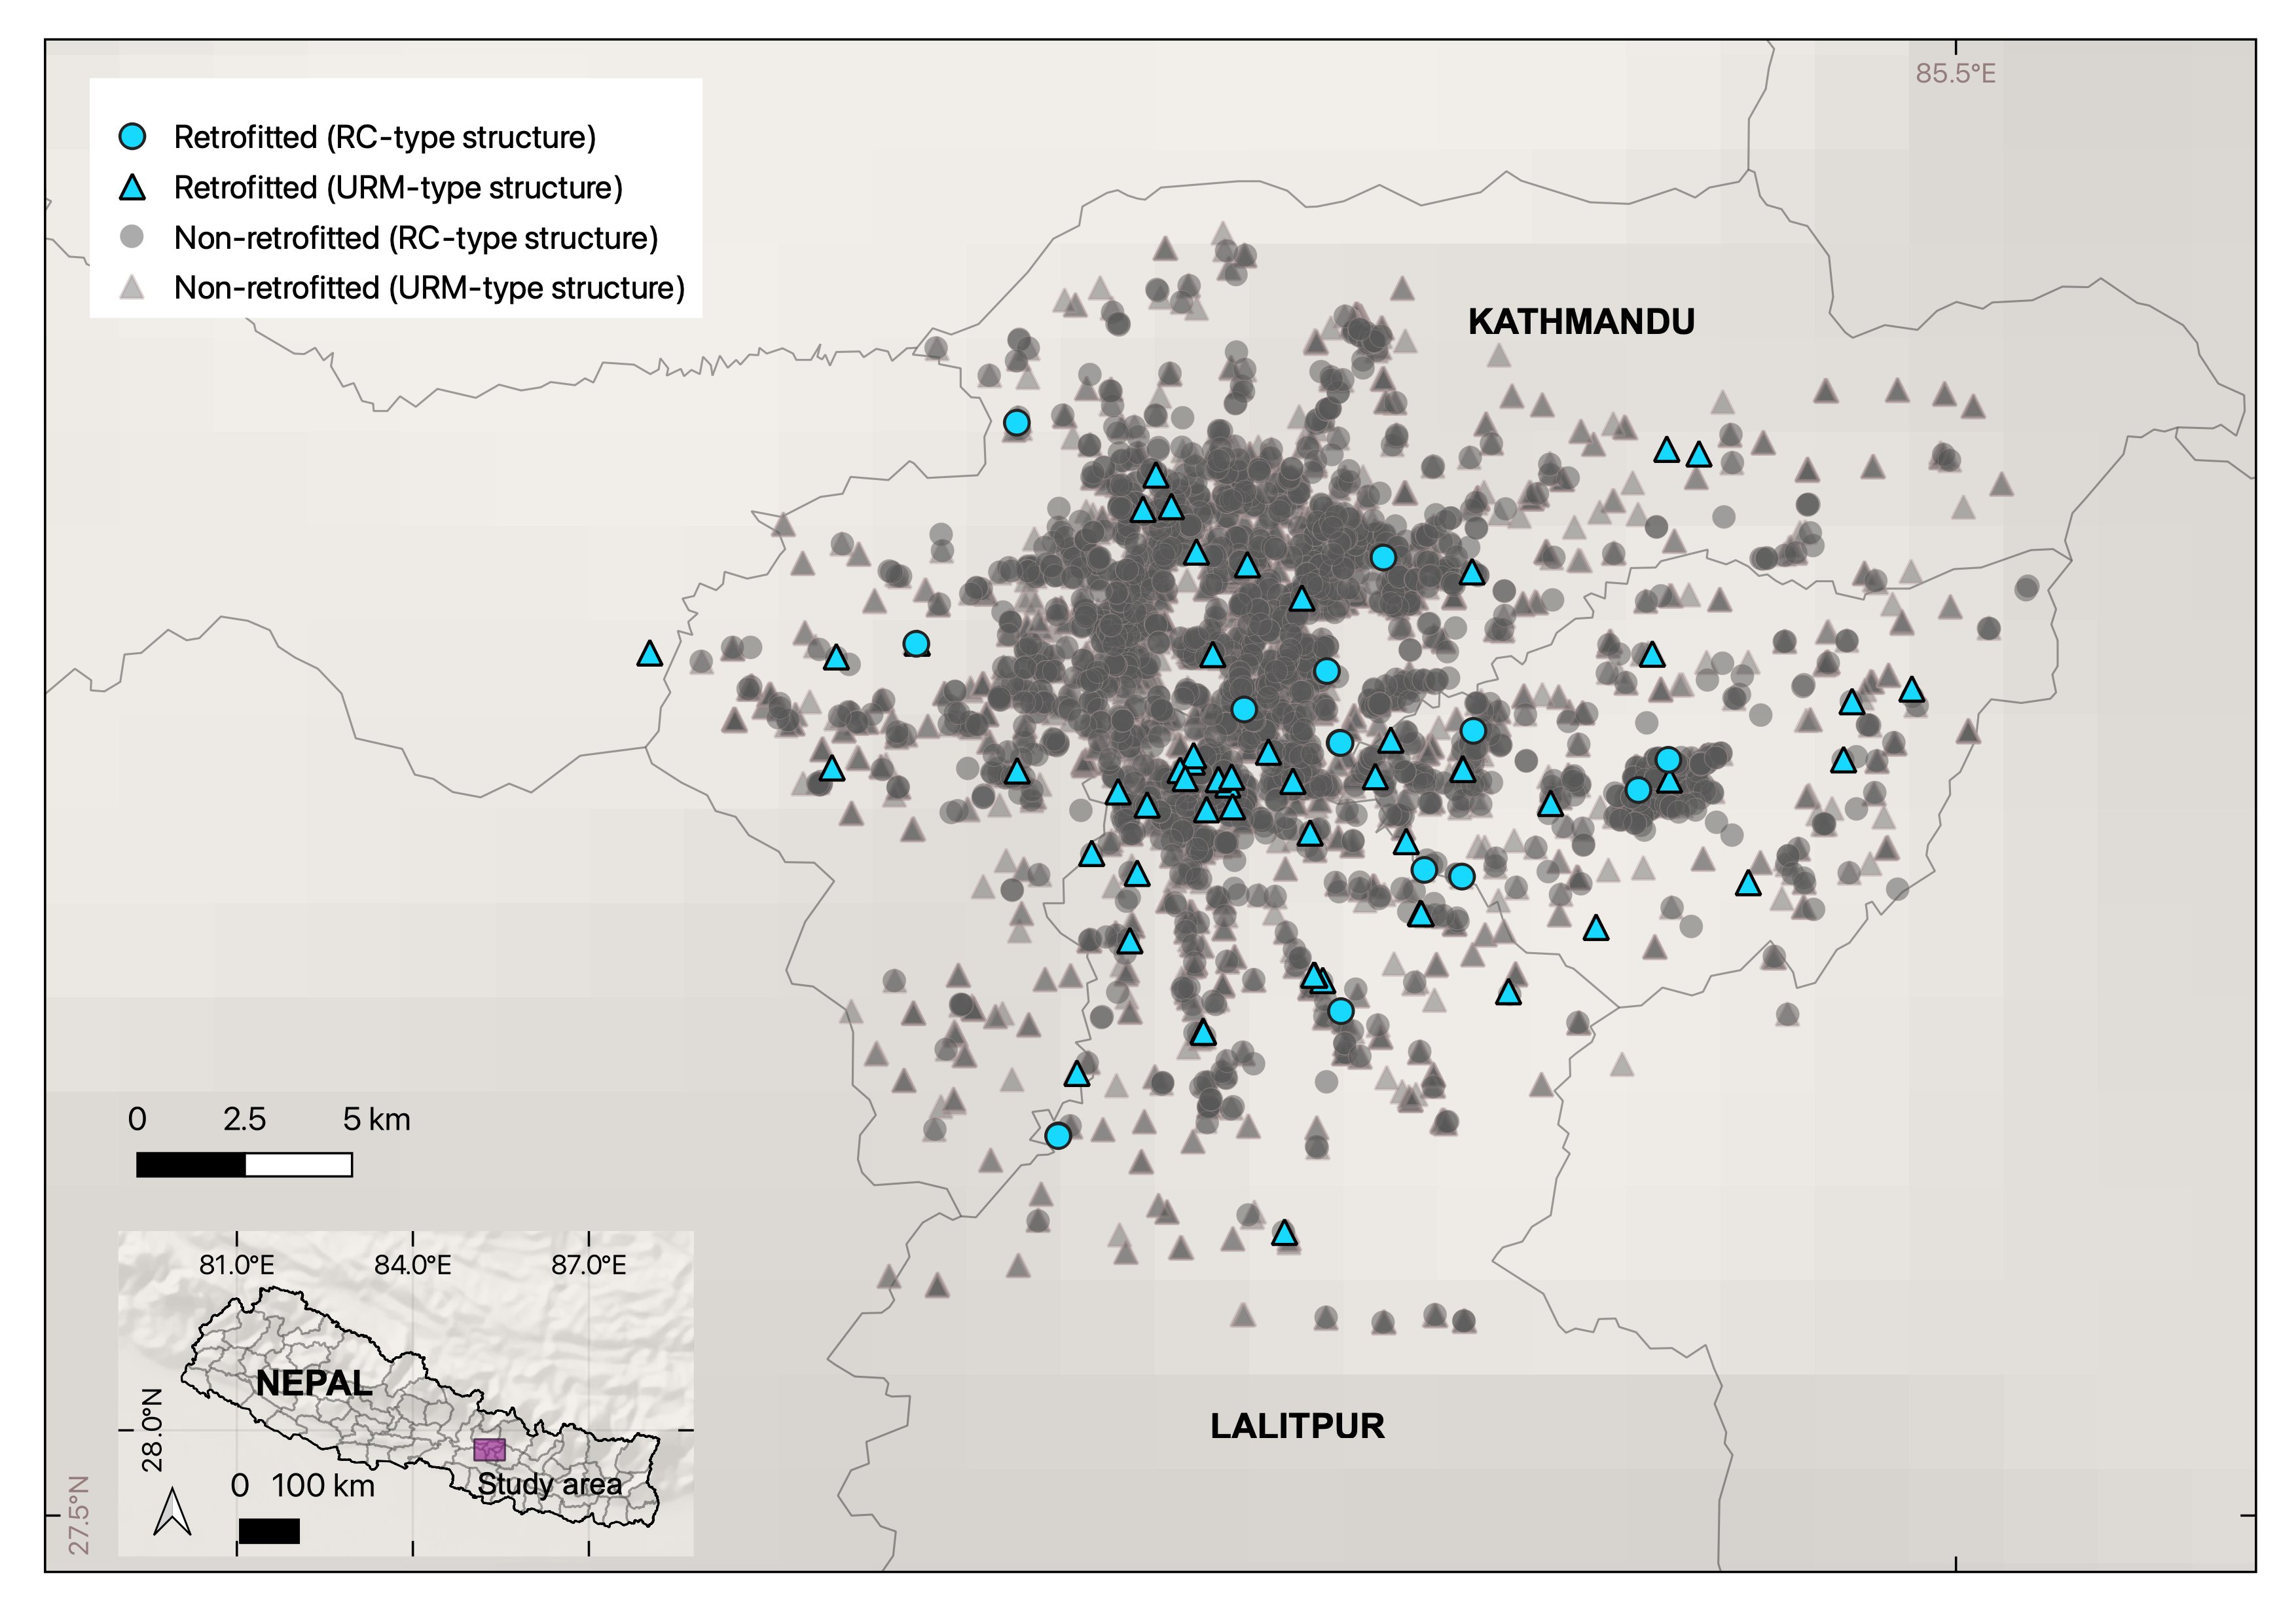
\includegraphics[width=\linewidth]{Figures/Datasets-basic.png}
	\caption{A map of the building database used in the analysis showing distribution of schools retrofitted and non-retrofitted as well as structure type.}
	\label{fig:data-all}
\end{center}
\end{figure}


\subsection{Building vulnerability modelling}
\label{section-vuln}

A fundamental step in estimating the benefit of a seismic retrofitting intervention involves obtaining the structure’s probability to exceed a certain damage level before and after the intervention. This paper focuses only on the collapse damage level since a vast majority of earthquake fatalities worldwide are due to building collapse \citep{spence2007saving}. Collapse fragility curves are used to represent the probability of collapse for a given earthquake intensity and building class. 

In this work, we have adopted collapse fragility curves developed by other authors to represent the probability of collapse of the buildings in their retrofitted and non-retrofitted states. The collapse fragility curves we use for the Nepalese school building stock in this study are presented in Figure \ref{fig:frag_curves}. The median $\eta$ and lognormal standard deviation $\beta$ of the fragility curves expressed as PGA lognormal distributions are shown in Table \ref{tab:frag_params}.

\begin{figure}[h!]
\begin{center}
    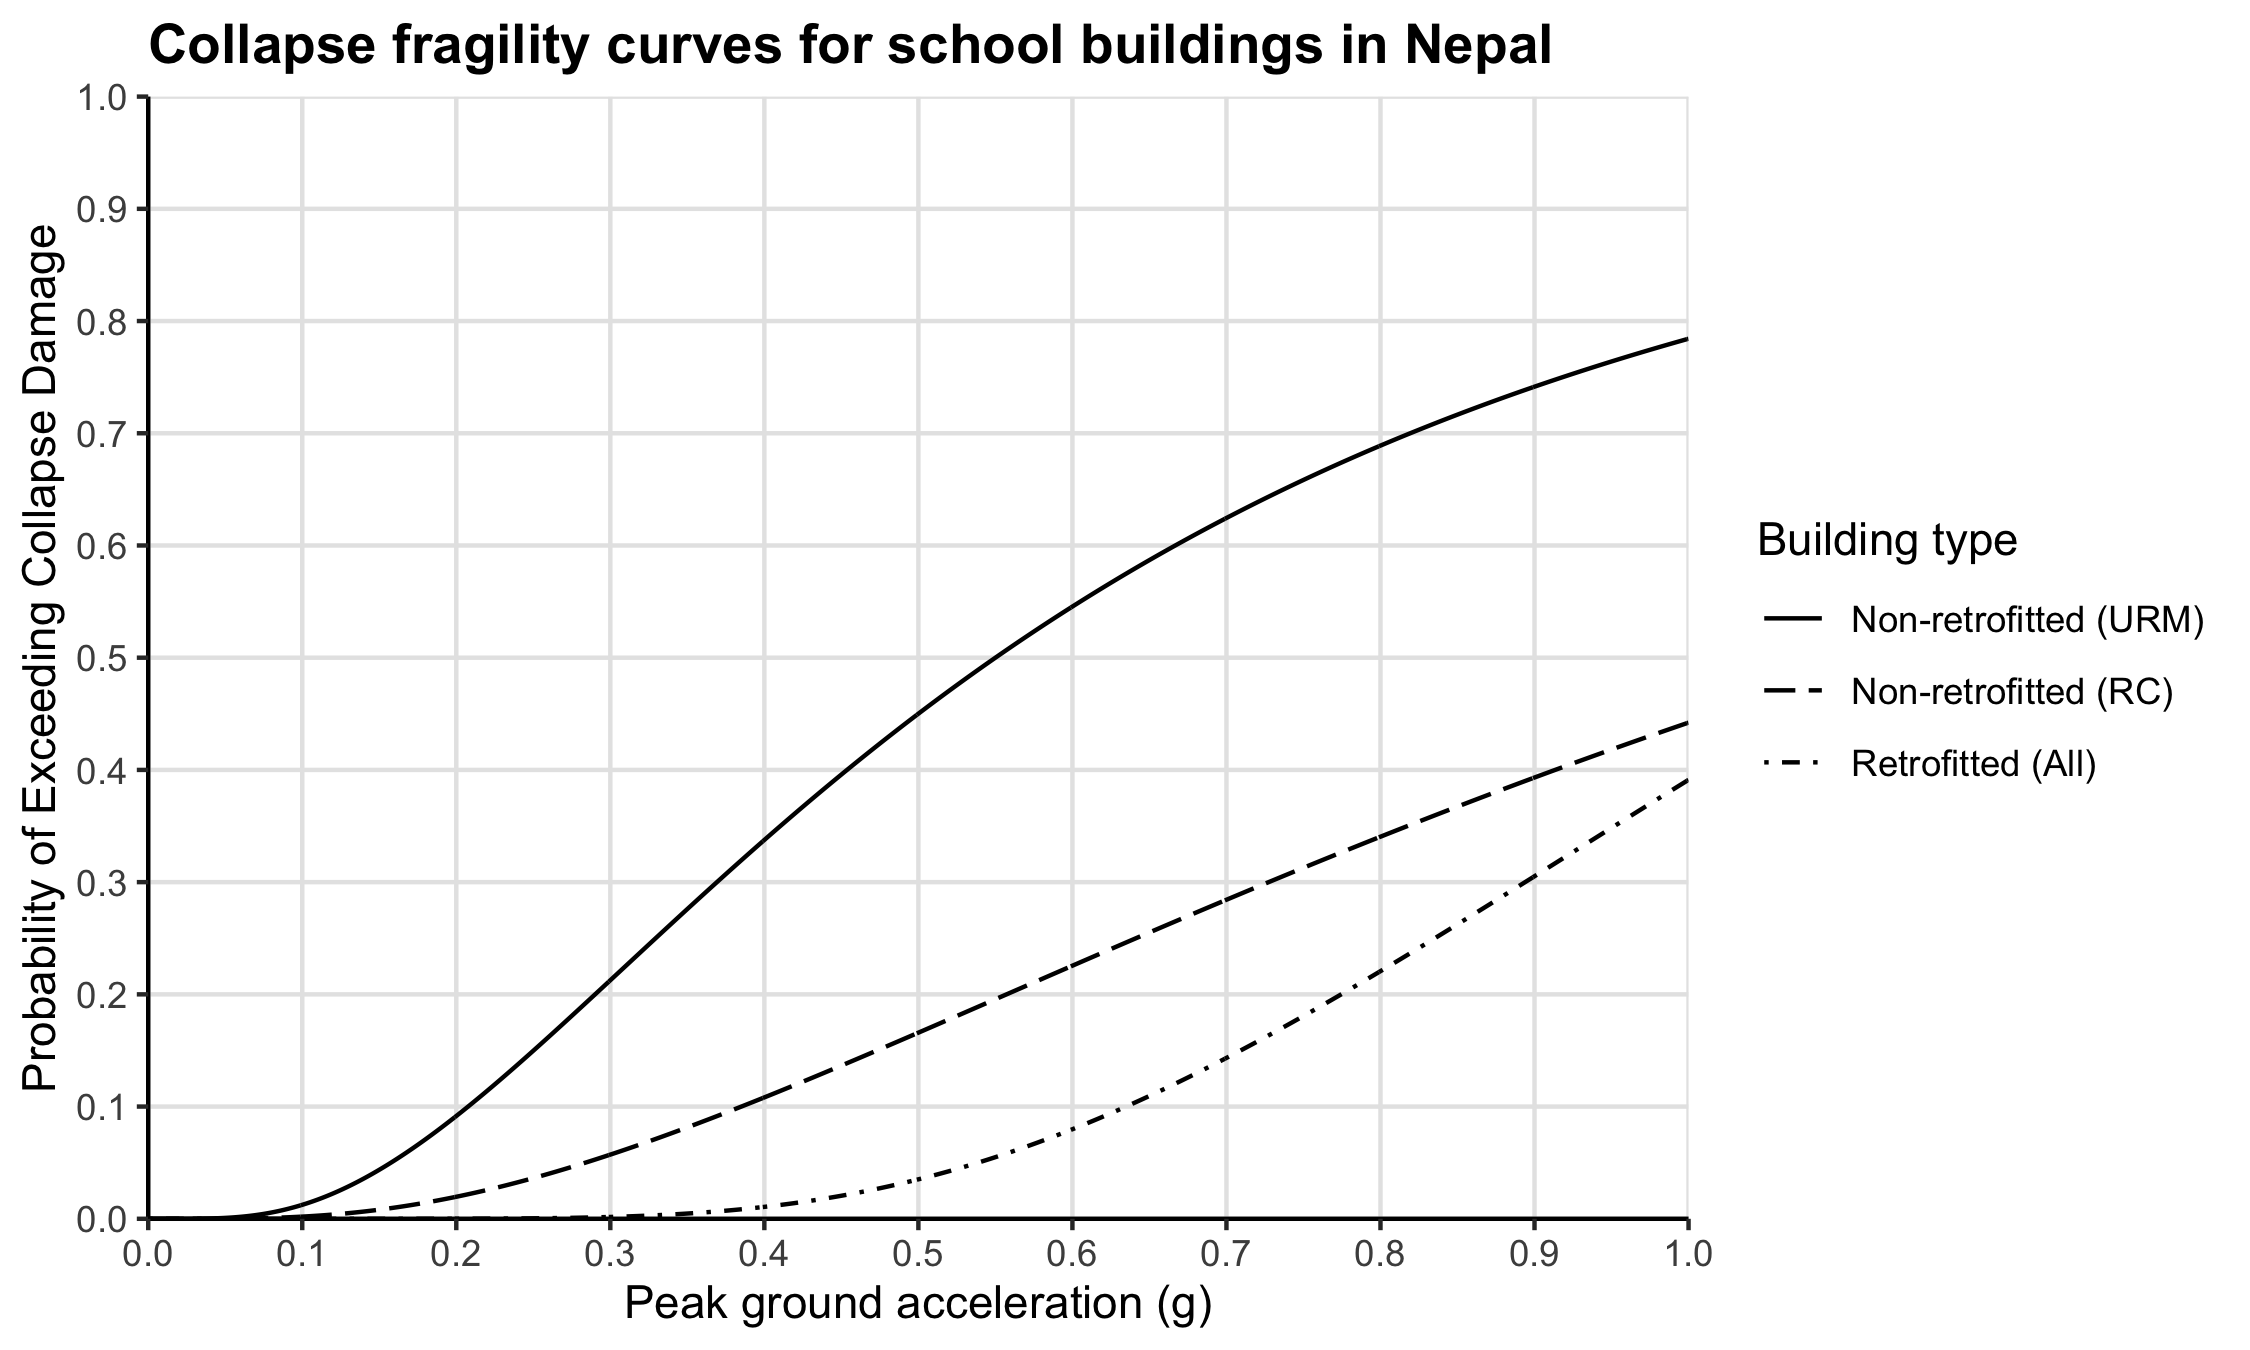
\includegraphics[width=\linewidth]{Figures/data-fragility-v4.png}
    \caption{Collapse fragility curves adopted in the analysis.}
    \label{fig:frag_curves}
\end{center}
\end{figure}

For non-retrofitted buildings, we adopt \cite{giordano2021empirical}'s empirical-based fragility curves specifically developed for Nepalese school buildings. The curves were generated using a Bayesian approach to incorporate well-established fragility models such as the HAZUS database \citep{mh20152} and World Bank's Structural Integrity and Damage Assessment database (SIDA) that was conducted under the Global Program for Safer Schools \citep{wbglosi}. The collapse fragility curves from \cite{giordano2021empirical} were assigned to the buildings in the OpenDRI dataset based on their structure type - unreinforced load-bearing wall schools were assigned the URM collapse fragility curve, while reinforced concrete schools were assigned the RC collapse fragility.

% Percent of URM and RC for total
% Insert assignment of building classes

For retrofitted buildings, we use the collapse fragility curve developed by \cite{giordano2021financial} for retrofitted stone masonry buildings in Nepal that are considered to have good quality material. The fragility curves in \cite{giordano2021financial} were produced analytically using a non-linear static pushover analysis for stone masonry buildings retrofitted with the 'RC strong-back approach'. It should be noted that the selected fragility curve for retrofitted school buildings does not necessarily represent the variation in the retrofit solutions available in Nepal, as well as the workmanship and original quality of the buildings, rather this is the best information available to the authors at the time of writing.

\begin{table}[]
\caption{Fragility curve parameters adopted in the analysis for the school buildings in the OpenDRI database. The parameters follow a lognormal model where $\eta$ (g) is the median PGA and $\beta$ is the lognormal standard deviation.}
\label{tab:frag_params}
\resizebox{\textwidth}{!}{%
\begin{tabular}{|c|l|c|c|c|}
\hline
    \multirow{2}{*}{\begin{tabular}[c]{@{}c@{}}Reference\end{tabular}} &
    \multicolumn{1}{c|}{\multirow{2}{*}{Building class}} &
    \multirow{2}{*}{\begin{tabular}[c]{@{}c@{}}Structural state \\ of building\end{tabular}} &
    \multicolumn{2}{c|}{\begin{tabular}[c]{@{}c@{}}Collapse state \\ parameters\end{tabular}} \\ \cline{4-5} 
        & \multicolumn{1}{c|}{}   &   & $\eta$  & $\beta$  \\ \hline
    \rule{0pt}{3ex}%  EXTRA vertical height  
            
    \citep{giordano2021empirical} &
    \begin{tabular}[c]{@{}l@{}}Non-retrofitted URM - Unreinforced masonry bearing wall,\\ low-rise (pre-code)\end{tabular} &
        Un-retrofitted &
        0.55 &
        0.76 \\ \hline
    \rule{0pt}{3ex}%  EXTRA vertical height  
            
    \citep{giordano2021empirical} &
    \begin{tabular}[c]{@{}l@{}}Non-retrofitted RC - Concrete frame buildings with\\ unreinforced masonry infill walls, low-rise (low code)\end{tabular} &
        Un-retrofitted &
        1.13 &
        0.84 \\ \hline
    \rule{0pt}{3ex}%  EXTRA vertical height    
            
    \citep{giordano2021financial} & Retrofitted stone masonry buildings      & Retrofitted    & 1.133 & 0.452 \\ \hline

\end{tabular}%
}
\end{table}            


\vspace{0.5cm} % because the paragraph space seems to small here

\subsection{Expected fatalities from building collapse}

A vast majority of earthquake fatalities worldwide are due to building collapse \citep{spence2007saving}. Therefore, this paper focuses on quantifying the fatalities from earthquake-induced building collapse, and the reduced estimated fatalities from retrofitting interventions.

To estimate fatalities due to building collapse, we adopt a semi-empirical casualty model that takes advantage of the availability of detailed building inventory and collapse fragility curves specific to the building types in Nepal. The approach is adopted from the semi-empirical forward model implemented in the USGS Prompt Assessment of Global Earthquakes for Response (PAGER) system \citep{jaiswal2011earthquake} for determining the extent of earthquake impacts globally. In contrast to USGS PAGER's use of Modified Mercalli shaking intensities, the earthquake intensity for this study is expressed in terms of peak ground accelerations. In this study, we calculate the total estimated fatalities $E[I]$ for a given building portfolio having a total number of $m$ buildings from a single earthquake event. Each building $i$ in the portfolio has a known structure type $k_{i}$. Using the empirical casualty model, we can write $E[I]$ as

    \begin{equation}\label{eq:loss_fat}
    E[I] = \sum_{i=1}^{m} O_{i} \cdot FR_{i}(k_{i}) \cdot C_{i}(im_{i}, k_{i})
    \end{equation} 
    %% per event based on stochastic 

where $O_{i}$ is the total exposed population inside building $i$ at the time of the earthquake, $FR_{i}(k_{i})$ is the fatality rate associated with the collapse of building $i$ based on its structure type $k_{i}$, and $C_{i}(im_{i}, k_{i})$ is the probability of collapse of building $i$ given the earthquake intensity at its location $im_{i}$ and its structure type $k_{i}$.

A fixed fatality rate of $FR_{i}(k_{i}) = 20\%$ for all structure types $k_{i}$ in the dataset is adopted for the study. This fatality rate is based on NSET's recommendation for both RC and masonry building classes, of which all the buildings in the dataset fall into \citep{nset2000}. This comes with an assumption that the same level of casualty is expected regardless of the level of school (e.g. primary or higher grades), nature of escape routes, or the occupants' level of preparedness.

By calculating $E[I]$ for a counterfactual and a realised scenario using Equation \ref{eq:loss_fat}, and plugging into Equation \ref{eq:benefits}, we can calculate the expected benefits of effective risk mitigation in terms of lives saved. In order to generate the entire probability distribution of fatalities, we conduct Bernoulli simulations (10,000) for collapse given a shaking intensity $C_{i}(im_{i})$ at each building location and for each building class $k_{i}$ for both the realised and counterfactual scenario. The complete source code is available at https://github.com/ntu-dasl-sg/frontiers2021-PLS.

 
%%%%%%%%%%%%%%%%%%%%%%%%%%%%|%%%%%%%%%%%%%%%%%%%%%%%%%%%%|
%%% APPLICATIONS
%%%%%%%%%%%%%%%%%%%%%%%%%%%%|%%%%%%%%%%%%%%%%%%%%%%%%%%%%|
\section{Applications}
\label{section-apps}

\subsection{Lives saved during the 2015 Gorkha earthquake due to the school retrofitting in Kathmandu Valley}
\label{section-case1}

In order to quantify the reduced fatalities from the school retrofit program in Kathmandu Valley, we estimate the fatalities during the 2015 Gorkha earthquake in the 70 retrofitted school buildings in our database as well as in the counterfactual scenario where these are not retrofitted. By chance, the earthquake occurred during a school holiday, during which occupancy was very low. For both re-analysis scenarios (current retrofit and counterfactual non-retrofit schools), we analyse fatalities for the expected occupancy during the school day. While there were a total of 160 schools retrofitted in  Kathmandu Valley at the time of the 2015 Gorkha earthquake \citep{marasini_2019}, our database contained information on 70. Hence while the focus of our analysis is on the life-saving benefit of the retrofit of the 70 schools in our data, the true reduction in fatalities due to the earthquake retrofitting program is much greater. A map of the 70 retrofitted school buildings used in this analysis is shown in  Figure \ref{fig:datacase1}.

\begin{figure}[h!] 
\begin{center}
    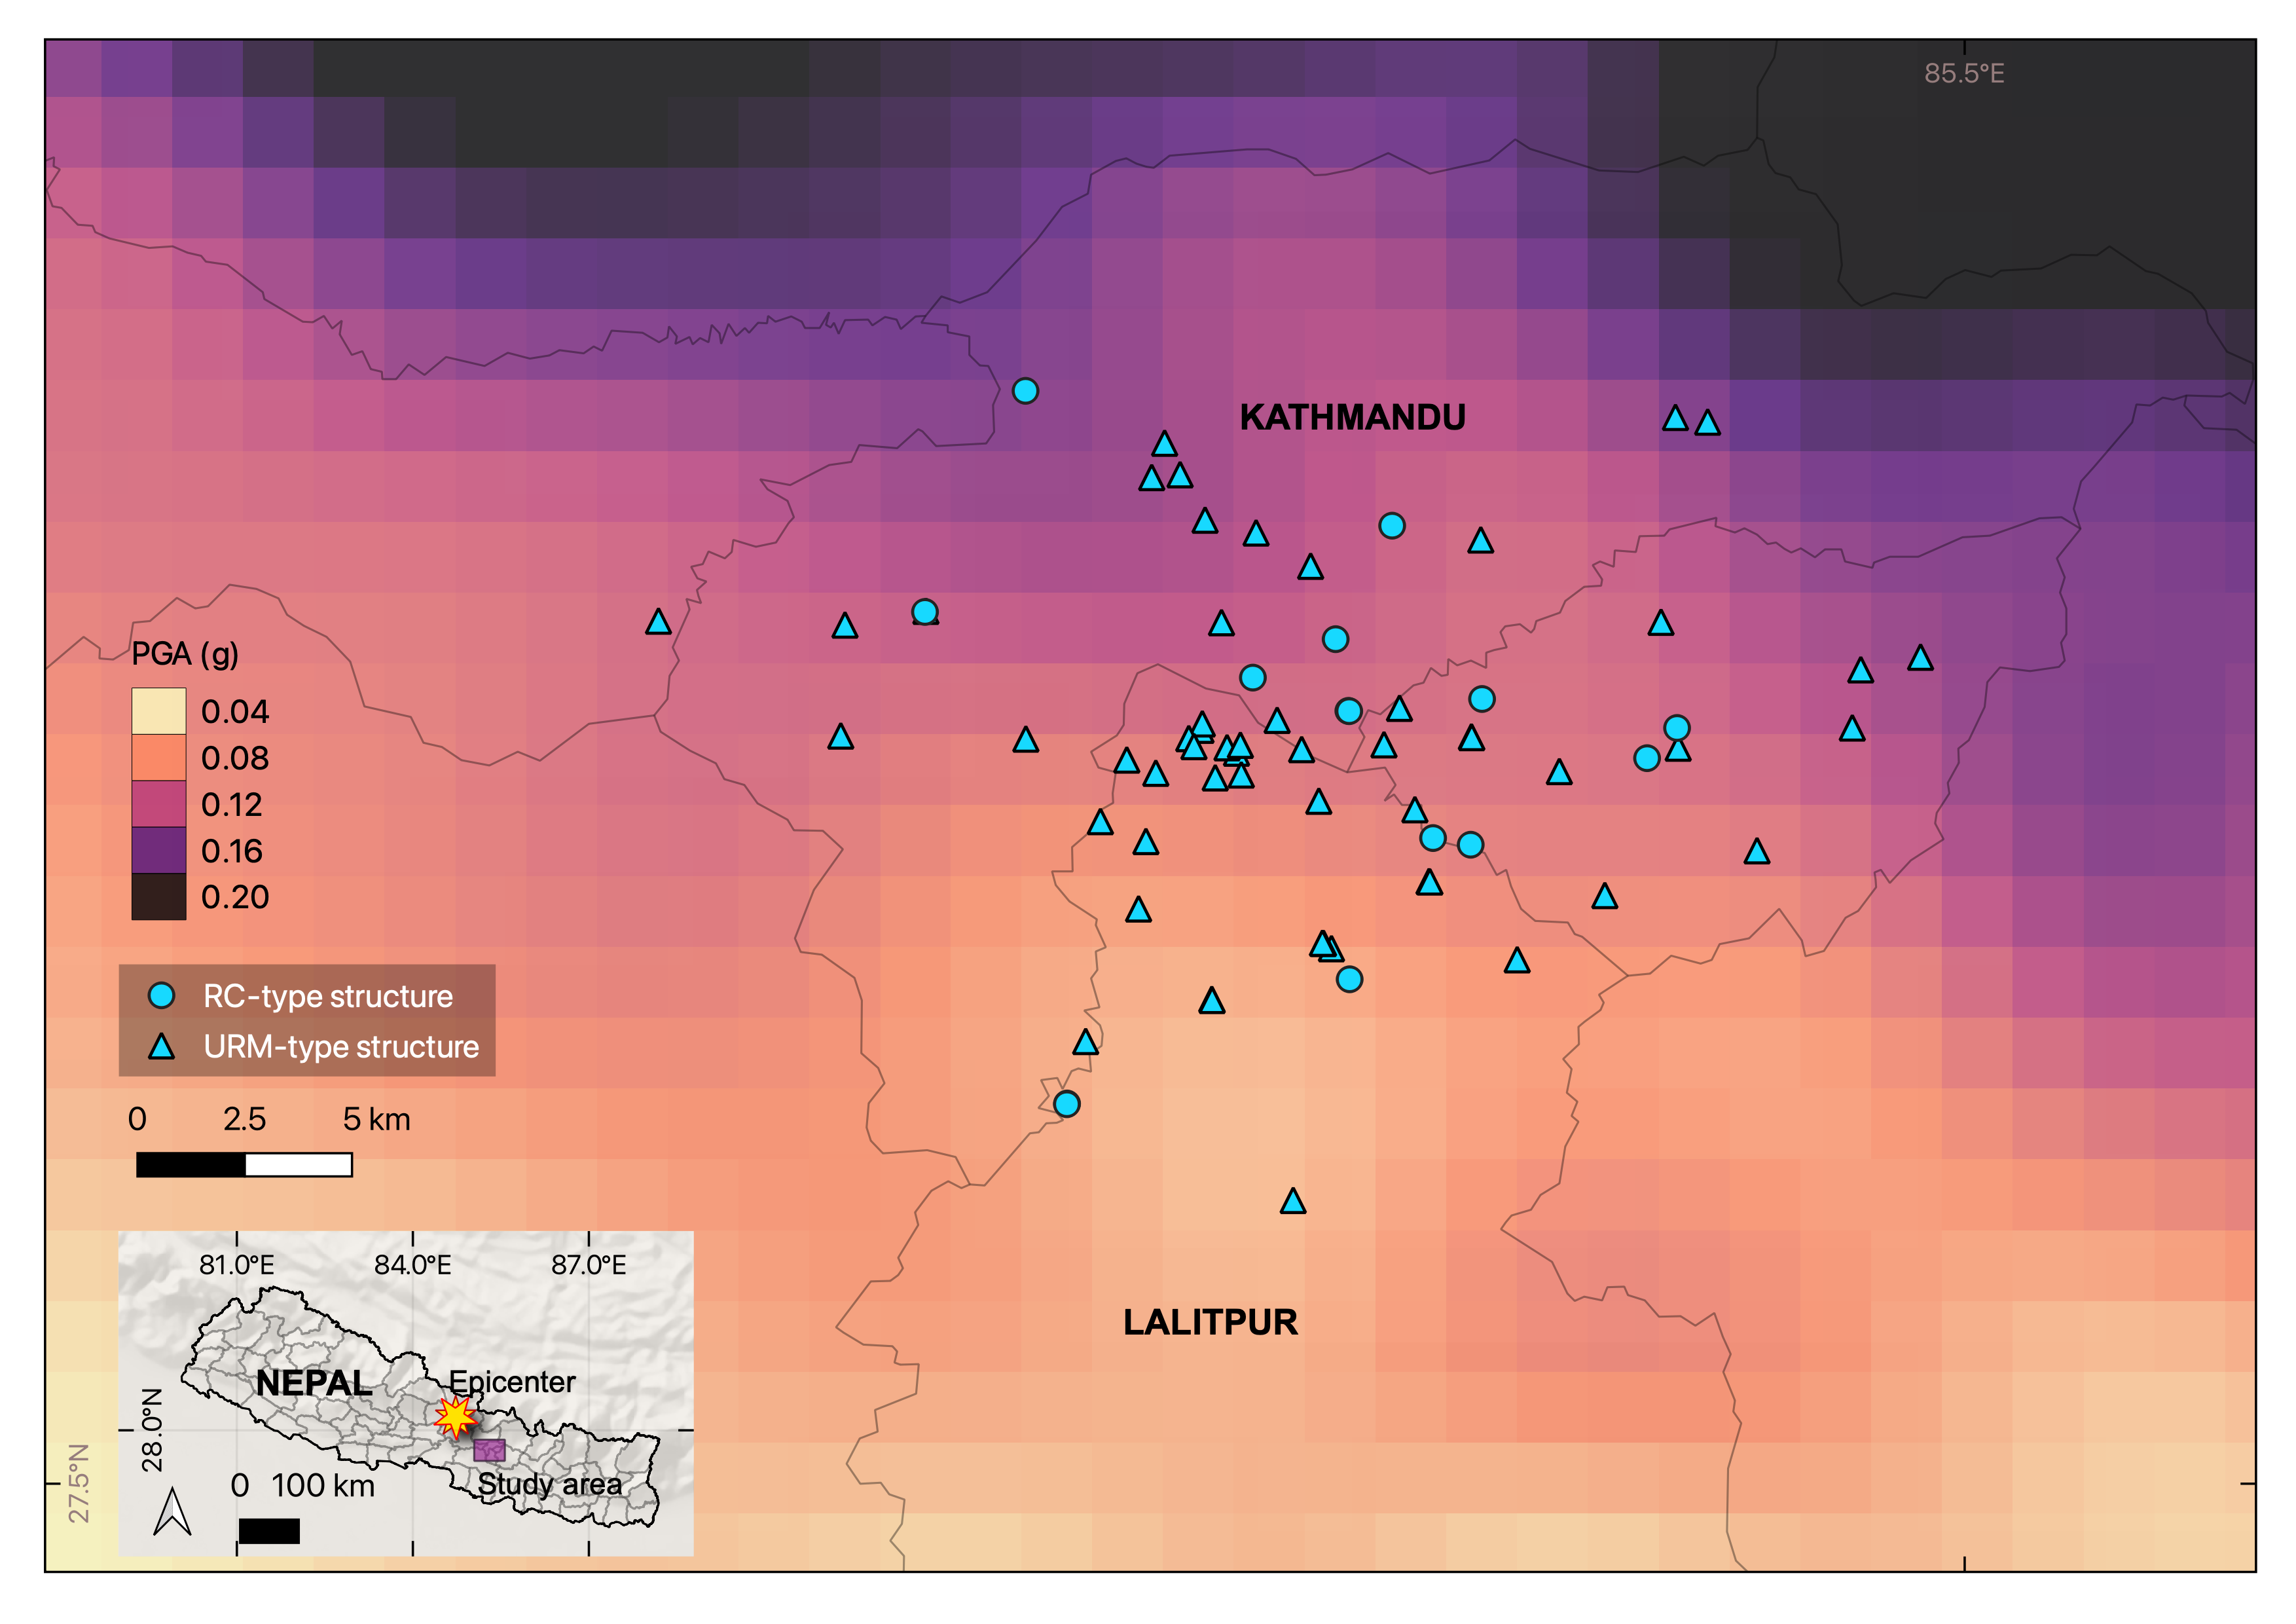
\includegraphics[width=\linewidth]{Figures/Dataset_Case1.png}
	\caption{A map of the 70 retrofitted schools and their corresponding structure type used in the analysis described in Section \ref{section-case1}. The basemap shows the hazard model developed by \cite{chen20192015} for the 2015 Gorkha earthquake in terms of peak ground acceleration (in g-units).}
	\label{fig:datacase1}
\end{center}
\end{figure}

The shaking intensity at the school sites during the 2015 Gorkha earthquake is obtained from the broadband ground-motion simulations produced by \cite{chen20192015} for the earthquake event. This hazard model was selected because the location of sources of the high-frequency energy (strong-motion generation areas) is a critical factor in explaining the relatively low damage phenomenon observed in Kathmandu Valley during the 2015 Gorkha earthquake \citep{gallovivc2016modeling, koketsu2016widespread}, aside from the effects of site conditions and rupture directivity \citep{dixit2015strong, rajaure2017characterizing, gallovivc2016modeling, koketsu2016widespread}. A map of the PGA values at the location of the retrofitted buildings is shown in Figure \ref{fig:datacase1}. With this hazard model, PGA values at the location of the retrofitted buildings range from 0.065 to 0.149 g, and come in a resolution of 0.0167 degrees, or around 1.85km.  More details about the PGA data are summarised in \cite{chen20192015} and its companion paper, \cite{wei20182015}.

In order to calculate the estimated impacts in a counterfactual scenario, $E[I]_{counterfactual}$, in which the SESP seismic retrofitting program was absent before the Gorkha earthquake, we use Equation \ref{eq:loss_fat} to estimate the total fatalities for the 70 buildings under this counterfactual scenario. The probability of collapse $C_{i}(im_{i}, k_{i})$ of any building $i$ is obtained from the fragility curve of the building at its \textit{non-retrofitted state} and the Gorkha earthquake event-specific PGA at the building's location $im_{i}$. The collapse fragility curves for the non-retrofitted state are assigned as described in Section \ref{section-vuln}, and the PGA values at the building locations are extracted from \cite{chen20192015}'s hazard model. Using these inputs in Equation \ref{eq:loss_fat} results to $E[I]_{counterfactual}$ = 25 fatalities.

The expected fatalities from the realised event $E[I]_{realised}$ can be calculated using the same approach, but using the collapse fragility curves corresponding to the \textit{retrofitted state} of the buildings as assigned in Section \ref{section-vuln}. This approach results in $E[I]_{realised}$ = 0 fatalities, which is the expected total number of fatalities in the realised scenario for the 70 buildings. By comparing the fatalities from the two scenarios as in Equation \ref{eq:benefits}, we estimate that the lives of approximately 25 school occupants were saved in Kathmandu by the retrofit of the 70 schools (see Figure \ref{fig:results_case1}).

\begin{figure}[h!] 
\begin{center} 
    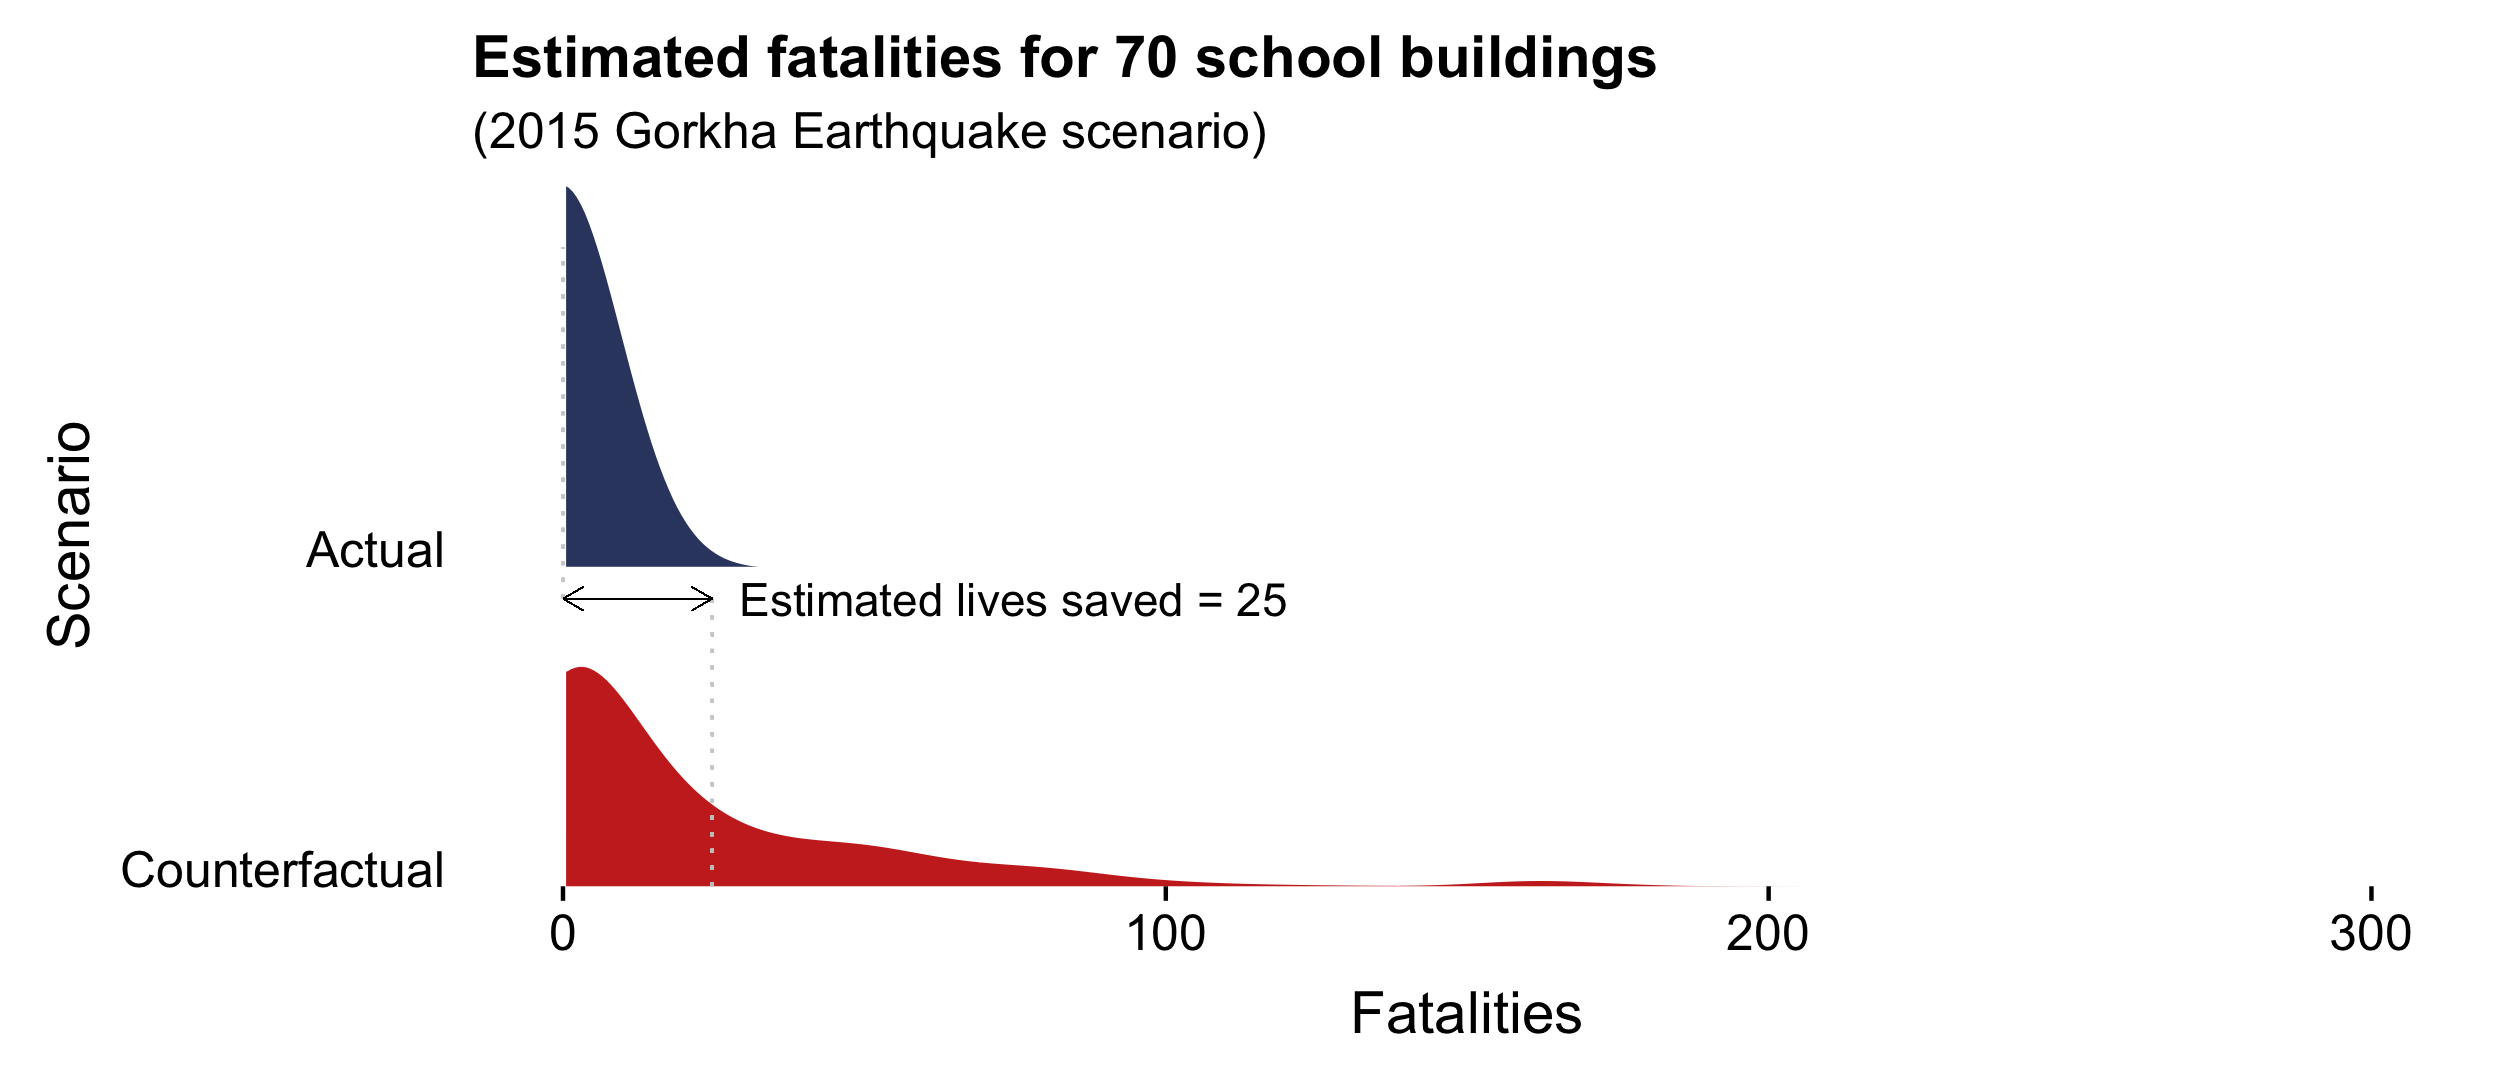
\includegraphics[width=\linewidth]{Figures/results_case1-v2.png}
	\caption{Distribution of estimated fatalities from the 2015 $M_{w}$ 7.8 Gorkha earthquake based on earthquake intensity values from \cite{chen20192015}. Two scenarios are shown: the actual scenario where all 70 school buildings were retrofitted prior to the 2015 Gorkha earthquake, and a counterfactual scenario where the schools were not retrofitted. Our analysis show an estimated 25 lives in the 70 retrofitted schools.}
\label{fig:results_case1}
\end{center}
\end{figure}

In an attempt to explore the sensitivity of the casualty estimates to different hazard models for the 2015 Gorkha earthquake, we repeated the analysis using a PGA map from the USGS ShakeMap \citep{shakemap2015nepal, wald2007topographic}. While using \cite{chen20192015}'s hazard model results in 25 lives saved, using the USGS ShakeMap hazard model results in 68 lives saved (see Figure \ref{fig:supplementary_ShakeMap} in the Appendix).  The analysis using either model highlights the life-saving benefit of the school retrofitting program, but we believe that the fatality analysis using \cite{chen20192015}'s model is more accurate in terms of representing the shaking during the 2015 Gorkha earthquake. \cite{chen20192015}'s model better captures the amplification or attenuation of the seismic shaking as it accounts for the location of sources of the high-frequency energy (strong-motion generation areas), rupture directivity, and site conditions critical in understanding the relatively low damage phenomenon observed in Kathmandu Valley during the earthquake. 

\vspace{0.5cm} % because the paragraph space seems to small here

\subsection{Annual expected lives saved through scaling the retrofit programs to all schools in Kathmandu Valley}
\label{section-case2}

Part of the Comprehensive School Safety Master Plan is the ambition to scale earthquake retrofitting to all vulnerable schools \citep{cehrdc2018}. As such, we develop a second case study to better understand the life-saving impact of such a program. We assess expected fatalities if the 5029 schools in Kathmandu Valley were retrofitted, and if they remained in their current state. This analysis is conducted for the entire seismic hazard of Nepal, to better reflect the distribution of potential events to impact Kathmandu Valley.

A probabilistic seismic hazard analysis (PSHA) was developed for the school building sites based on twenty-three independent seismic source zones for Nepal identified by \cite{ram2013probabilistic} and adopted in \cite{chaulagain2015seismic}’s PSHA model. The ground motion prediction equation by \cite{chiou2014update} for active shallow crust regions is used within a logic tree for an event-based probabilistic seismic hazard calculation in the OpenQuake-engine \citep{silva2014development}. To reach statistical convergence, 100,000 stochastic event sets with a 1-year time interval were generated \citep{silva2016critical}. The result of the simulation is a large number of realisations of seismic events and corresponding shaking at the locations of the schools within a year. The resulting hazard curves for some selected schools in the database are shown in Figure \ref{fig:hazcurve}.

\begin{figure}[h!] 
\begin{center}
    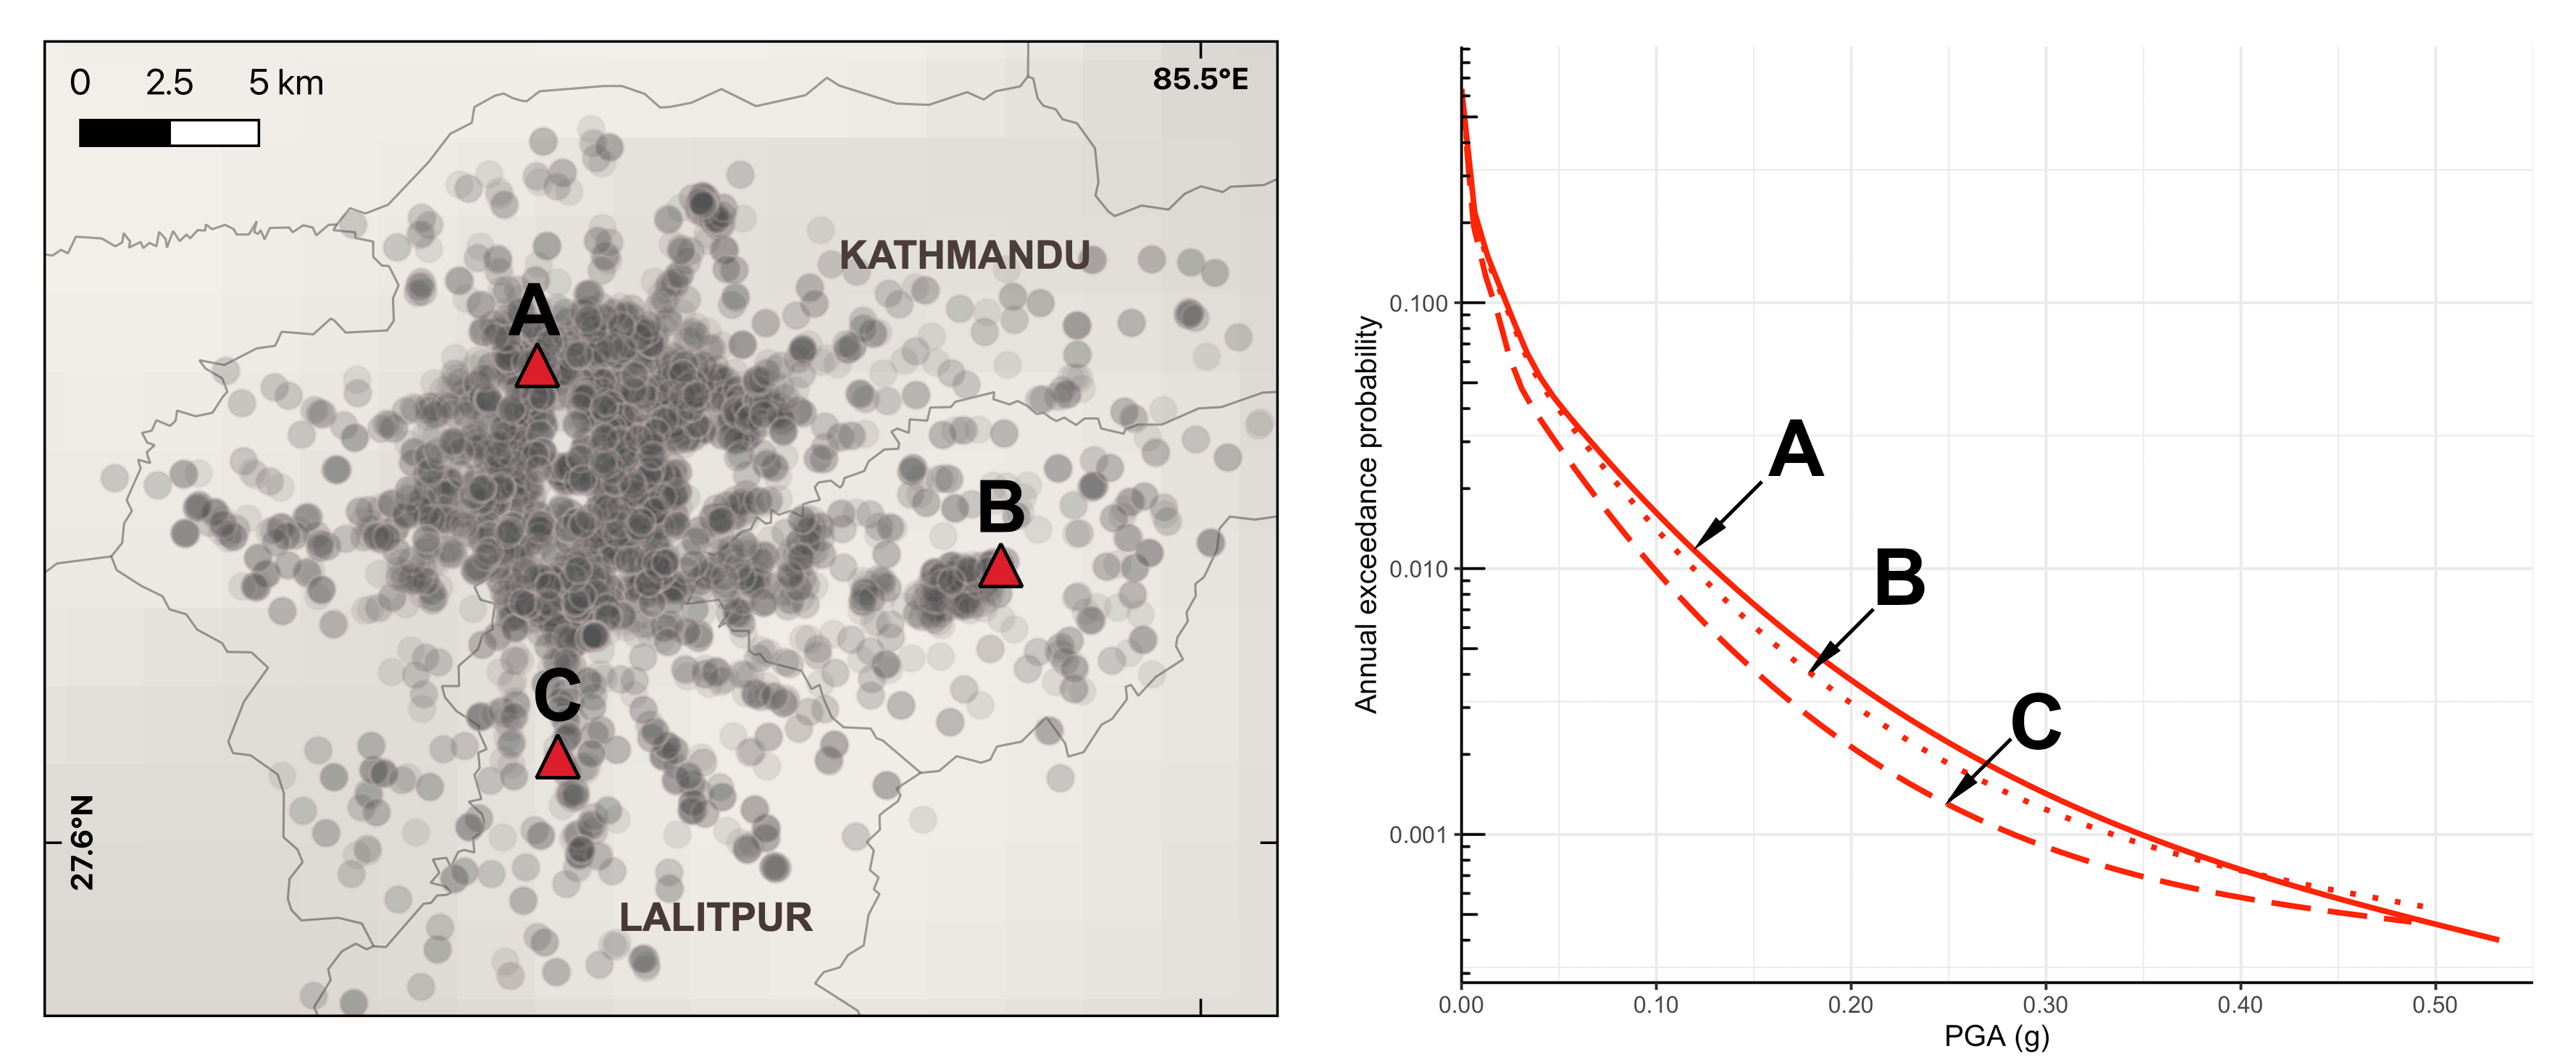
\includegraphics[width=\linewidth]{Figures/hazcurves-v5.png}
	\caption{Hazard curves for three sample school building locations in the analysis.}
	\label{fig:hazcurve}
\end{center}
\end{figure}

For every event generated, the number of fatalities in the building portfolio due to collapse is estimated using Equation \ref{eq:loss_fat}. In the fatality calculation of each event, we incorporate the probability distribution of school building occupancy. In Nepal, schools are open and run 220 days a year, and each school day lasts for 6 hours \citep{nepal2009reform}. This means that out of the 8760 hours in a year, 1320 (15\%) are school hours in Nepal. To account for this, we simulate a large number of Bernoulli trials for each event that takes a 15\% probability of occurring during school hours. The resulting annual fatality exceedance probability curves for two different retrofitting scenarios are shown in Figure \ref{fig:losscurve}. The fatality calculation in this study assumes no uncertainty related to the time of the day during school hours. This means that the building occupancy is constant during school hours, whereas outside school hours, the building occupancy is 0.

\begin{figure}[h!] 
\begin{center}
    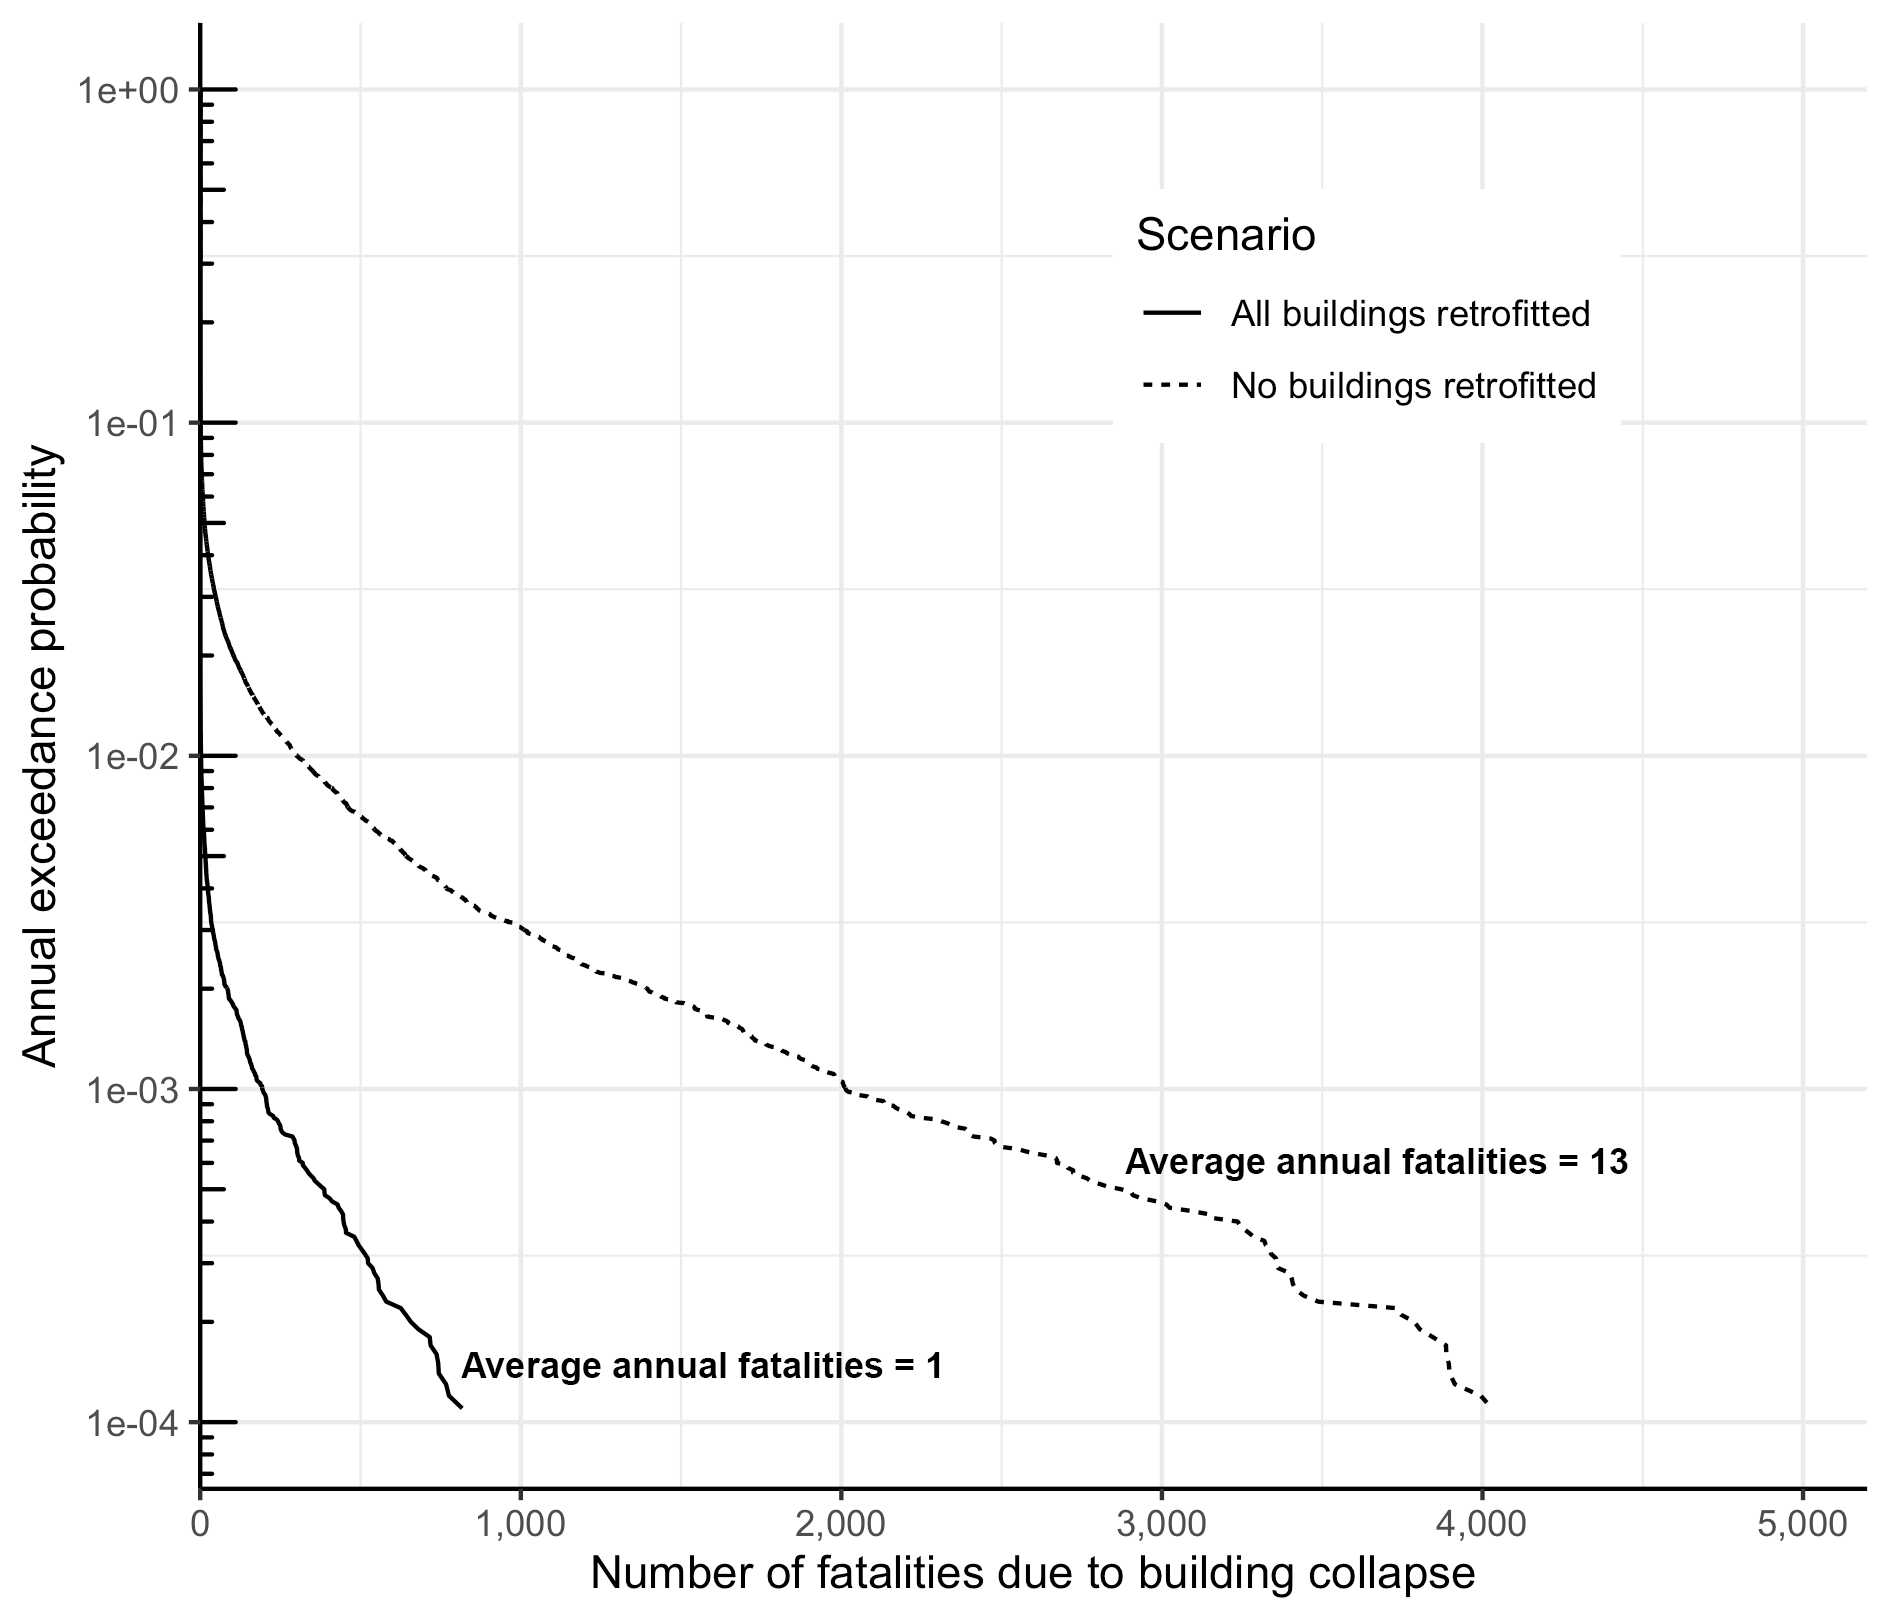
\includegraphics[width=\linewidth]{Figures/loss_curve_ALL_100k-annotate.png}
	\caption{Benefits of extending Nepal's school retrofit program to 5029 schools in the database in terms of the shift in the annual fatality exceedance curve.}
	\label{fig:losscurve}
\end{center}
\end{figure}

The average annual fatalities are obtained by integrating the integrating the annual fatality exceedance probability curve. For the scenario in which none of the 5029 school buildings is retrofitted, we estimate 13 average annual fatalities, whereas when the retrofitting program is extended to all buildings, we estimate an average of 1 annual fatality. In this probabilistic analysis, we calculate an average of 12 annual lives saved from scaling the retrofit program in all of Kathmandu Valley.
%%%%%%%%%%%%%%%%%%%%%%%%%%%%|%%%%%%%%%%%%%%%%%%%%%%%%%%%%|
%%% CONCLUSION
%%%%%%%%%%%%%%%%%%%%%%%%%%%%|%%%%%%%%%%%%%%%%%%%%%%%%%%%%|
\section{Discussion}
\label{section-discussion}

\subsection{A counterfactual analysis approach to celebrate effective risk reduction}

In a field focused on long-term resilience to rare (i.e. volatile) hazard events, perceptions of risk are biased by realised outcomes. The perception of \textit{no impacts} when in fact DRM work is successful can result in policymakers and society at large to undervalue the importance of proactive intervention. Shedding light on successes and \textit{what might have been}, not only recognizes the outstanding work of those working to reduce risk, but is also a crucial component of encouraging decision-makers to continue investments in measures that keep our communities safe. 

We highlight the need to celebrate the often invisible successes of disaster risk reduction interventions, in order to incentivise, better learn and replicate investments in such interventions. We further propose and demonstrate the use of a probabilistic counterfactual risk analysis framework to identify, quantify and highlight these invisible successes. The framework demonstrates that judgement of a risk reduction intervention should be based on a broad exploration of possible outcomes, not only on specific outcomes.

We demonstrated two applications of the probabilistic downward counterfactual risk analysis to (1) celebrate lives saved by a disaster risk reduction intervention (earthquake school retrofitting) amidst a past event (the 2015 Gorkha earthquake in Nepal), and (2) assess expected annual lives saved due to the intervention with the use of a probabilistic hazard model. The two applications show that even in the midst of a tragic disaster, or if a hazard event has not occurred yet, there are often successes in risk reduction intervention to celebrate. The counterfactual analysis showed that numerous expected fatalities were avoided during the Gorkha earthquake because of the government-led retrofitting of school buildings starting in 1997, and many more could be saved if the retrofit program were scaled to all schools in Kathmandu Valley. 

\vspace{0.5cm} % because the paragraph space seems to small here

\subsection{Lives saved as a risk reduction benefit metric}

In our demonstrations, the risk benefit of DRM intervention is measured in terms of a reduction in loss of life - the first target metric within the Sendai Framework For Disaster Risk Reduction \citep{united2015sendai}. A risk benefit metric in financial units can also be used, as with a typical cost-benefit analysis. However such analysis tends to highlight interventions that effectively protect high-value areas instead of high-vulnerability areas, which exacerbates inequities \citep{markhvida_quantification_2020, lallemant2020informatics}. 

More alternative risk reduction benefit metrics for this analysis include the number of displaced people, business downtime, damage to buildings and cultural heritage, psychological distress and more. For the Nepal case study, for example, the benefits of retrofitting go well beyond the reduced physical vulnerability of the buildings. Retrofitted schools served as immediate community shelters, field hospitals and relief centres. Classes in the retrofitted buildings were operated without fear, resulting in less demand for temporary classrooms \citep{marasini2020}. Loss avoidance is not the only invisible benefit of disaster mitigation, and the benefits of DRM interventions go beyond reduction of impact. Certain intervention designs can have co-benefits such as retrofit programs that improve the environmental comfort of classrooms, that serve as training platforms to local constructors who replicate the methods in other building constructions, or that are linked with student and teacher earthquake preparedness programs \citep{spence2021buildings}.

\vspace{0.5cm} % because the paragraph space seems to small here

\subsection{First order approach}

The analyses and estimates of lives saved presented are first order and serve as proof of concept of the counterfactual framework to highlight successes in DRM. Following are limitations that need to be noted for future work:

\begin{itemize}
    \item 
    The analysis did not account for fatalities from partially collapsed buildings. To account for this, one may use NSET's recommendation to use a 10\% fatality rate for heavily damaged buildings \citep{nset2000}
    \item
    The building portfolio dataset we use in the two case studies is only a subset of all the schools within the study area. The dataset used for the first case study (Section \ref{section-case1}) contains only 70 out of the 160 retrofitted schools in Kathmandu Valley. For the second case study (Section \ref{section-case2}), we also did not include school building data that has no information on the occupancy and structure type.
    \item
    For the second case study, the assumption that all 5,029 school buildings will be retrofitted seems in line with the plans of the Government of Nepal. However, it is not a forecast of the future, as much uncertainty remains. We hope that our analysis serves to support policy decisions for more resilient schools.
\end{itemize}

\subsection{Broader applications with other domains of hazard and interventions}
\label{subsec-broadapps}

Probabilistic downward counterfactual risk analysis has potential for application to other hazards. A key step of the framework is to identify which risk component the intervention influences. Earthquake risk reduction, for example, influences either the reduction of exposure or vulnerability. Measures such as restricting development in high-hazard zones decrease exposure, whereas better construction standards decrease the structural vulnerability of buildings and infrastructure.

Beyond earthquake risk reduction, the proposed framework can also be used in other domains of hazard. Following are a few selected examples of natural hazards and corresponding interventions that could be celebrated using counterfactual analysis. Enclosed in parenthesis are the risk component/s that the intervention influences.

\begin{enumerate}

    \item \textbf{Earthquake}
    \begin{itemize}
            \item Reconstruction and seismic retrofit (Vulnerability)
            \item Construction inspection (Vulnerability)
            \item Preparedness exercises (Exposure, Vulnerability)
    \end{itemize}
    
    \item \textbf{Tropical cyclone and Tsunami}
    \begin{itemize}
            \item Early warning system and timely announcements (Exposure)
            \item Evacuation and provision of temporary shelters (Exposure and Vulnerability)
            \item Public awareness about the hazard (Exposure and Vulnerability)
    \end{itemize}
    
    \item \textbf{Flood}
    \begin{itemize}
            \item Limiting urban development in flood-prone zones (Exposure, Vulnerability)
            \item Enhanced flood management infrastructure (Exposure, Hazard)
            \item Timely emergency response (Vulnerability, Exposure)
            \item Preservation or restoration of natural ecosystems for flood mitigation (Hazard)
    \end{itemize}

    \item \textbf{Landslides}
    \begin{itemize}
            \item Early warning system via geodynamic monitoring (Exposure)
            \item Mitigation infrastructure, e.g. drainage systems (Exposure, Hazard)
    \end{itemize}

    \item \textbf{Wildfires}
    \begin{itemize}
            \item Early warning system via dynamic weather forecasts (Exposure)
    \end{itemize}

\end{enumerate}


\section{Conclusion}
\label{section-conclusion}

This study combines the probabilistic risk analysis framework and counterfactual analysis to quantify and highlight the significant benefits of successful disaster risk reduction interventions that often go unnoticed. By using an appropriate counterfactual scenario as a baseline against which to compare realised outcomes, it makes clear that the impact of hazards would be much worse without important investments in risk reduction.

Using this approach, we demonstrate that an estimated 25 lives were saved (probabilistically) during the 2015 Gorkha earthquake from the retrofitting of 70 schools in Kathmandu Valley alone. If such a retrofitting program were scaled to all the approximately 5,029 schools in Kathmandu Valley, we estimate a reduction of 12 annual school children fatalities based on the significant seismic hazard of the region. These are clearly important programs that should be prioritized, celebrated, scaled, and replicated in areas with high seismic risk.

Loss of life reduction is an important metric for risk reduction, not only because the life-safety of children and all people is paramount, but also because doing so centres attention on high-vulnerability areas and buildings, even if the financial losses associated may be small. However loss-avoidance is not the only invisible benefit of disaster mitigation, and the many co-benefits can also be included to further highlight the value of risk reduction interventions.

While this study demonstrates the application of probabilistic counterfactual risk analysis to quantify the life-saving value of a school earthquake retrofitting program in Kathmandu Valley, the methodology can be used in other contexts and hazards. Programs for typhoon and tsunami early warning, hazard informed urban development planning, flood-management through nature-based solution are all examples of important programs whose true benefits could be more accurately valued through the use of probabilistic counterfactual analysis. In so doing, such analysis would provide increased incentives to invest in risk reduction programs, learn from ones with demonstrated success, and serve to encourage those whose humble work is critically important even when often unnoticed.


%----------------
\section{Code and data availability}
%----------------
The complete source code for the analysis is written in the R Programming language  (R 4.0.2, \cite{team2013r}). All code and data for the study presented in this chapter is available at at https://github.com/ntu-dasl-sg/frontiers2021-PLS. 

%%%%%%%%%%%%%%%%%%%%%%%%%%%%
\section{Funding}
This project is supported by the National Research Foundation, Prime Minister’s Office, Singapore under the NRF-NRFF2018-06 award, the Earth Observatory of Singapore, the National Research Foundation of Singapore, and the Singapore Ministry of Education under the Research Centers of Excellence initiative. MR is supported by a PhD scholarship from the Earth Observatory of Singapore.

%%%%%%%%%%%%%%%%%%%%%%%%%%%%
\section{Acknowledgments}
We thank Dr. Nama Budhathoki, Kathmandu Living Labs and the GFDRR Open Data for Resilience Initiative for data on school buildings in Nepal. We also thank Dr. Shengji Wei and Dr. Meng Chen for data and information on the broadband simulations in Kathmandu for the 2015 Gorkha earthquake, and Dr. Michele Nguyen for the guidance on the use of the OpenQuake engine.
